\documentclass[letterpaper,10pt]{book}
% Change to 10 pt
\usepackage{pdfpages}
\usepackage{morewrites}			% to counteract the no write space problem
\setcounter{tocdepth}{6}

\usepackage[framemethod=TikZ]{mdframed}

\usepackage{fancyhdr}

\usepackage{paralist}
\usepackage{amsmath}
\usepackage{amsfonts}
\usepackage{amssymb}
\usepackage{graphicx}

\usepackage{datetime}
%\usepackage{ulem}

%\usepackage[nottoc]{toobibind}

\usepackage[inline]{enumitem}

% Outer margin at 2.50 is exacty correct to fit the ``corruption alert'' tables
\usepackage[inner=1.0in, outer=2.50in, top=2.54cm,bottom=2.54cm, marginparwidth=2.25in]{geometry}

\usepackage{marginnote}
\usepackage{longtable}
\usepackage{booktabs}
\usepackage{xcolor}

\usepackage{soul}

%%%%%%%%%%%%
\definecolor{ForestGreen}{rgb}{0.00,0.29,0.098}
%%%%%%%%%%%%

\usepackage{marginnote}

\usepackage{imakeidx} 
\usepackage[
	backref=true,
	style=numeric,
%	citestyle=numeric,
	backend=bibtex
	]{biblatex}
\usepackage[driverfallback=hypertex,colorlinks=True]{hyperref}
\usepackage{cleveref}

\makeindex[name=scripture,columnsep=20pt, columnseprule=True,columns=3, title=Scripture References]
\makeindex[name=speaker,columnsep=20pt, columnseprule=True,,columns=2, title=Sermon Creator]
\makeindex[name=series,columnsep=20pt, columnseprule=True,,columns=2, title=Sermon Series]
\makeindex[name=date,columnsep=20pt, columnseprule=True,columns=2, title=Sermon Date]
\makeindex[name=event,columnsep=20pt, columnseprule=True,columns=2, title=Event]
\makeindex[name=topic,columnsep=20pt, columnseprule=True,columns=2, title=Topic]
\makeindex[name=AWIP,columnsep=20pt, columnseprule=True,columns=3, title=All Words in Passage]
\makeindex[name=NWIV,columnsep=20pt, columnseprule=True,columns=3, title=Number of Words in Verse]
\makeindex[name=PNIP,columnsep=20pt, columnseprule=True,columns=3, title=Proper Names in Passage]
\makeindex[name=PEIP,columnsep=20pt, columnseprule=True,columns=2, title=Prophetic Events in Passage]
\makeindex[name=TWPAQ,columnsep=20pt, columnseprule=True,columns=1, title=13-Word Phrases and Quotes]
\makeindex[name=PFTTIS,columnsep=20pt, columnseprule=False,columns=3, title=Phrases found 13 times in scripture]
\makeindex[name=WFTTIS,columnsep=20pt, columnseprule=False,columns=3, title=Words found 13 times in scripture]
\makeindex[name=WFITV,columnsep=20pt, columnseprule=False,columns=3, title=Words found in exactly 13 verses]
\makeindex[name=EVENTS,columnsep=20pt, columnseprule=False,columns=2, title=Sermon Log by Place]
\makeindex[name=QUESTIONS,columnsep=20pt, columnseprule=False,columns=2, title=Bible Questions]
\makeindex[name=DOCTRINES,columnsep=20pt, columnseprule=False,columns=2, title=Doctrines]
\makeindex[name=SONGS,columnsep=20pt, columnseprule=False,columns=1, title=Songs]
\makeindex[name=LOCATION,columnsep=20pt, columnseprule=False,columns= 2, title=Location]
\makeindex[name=FACEBOOK,columnsep=20pt, columnseprule=False,columns=2, title=Facebook]
\makeindex[name=DEVOTIONAL,columnsep=20pt, columnseprule=False,columns=2, title=Devotional Items]
%%%%%%%%%%%%%%%%% EXTRA COLORS
\definecolor{champagne}{rgb}{0.97,0.91,0.81}
\definecolor{bone}{rgb}{0.89,0.85,0.79}
\pagestyle{fancy}
\fancyhf{}
\fancyhead[LE,RO]{\today}
\fancyhead[RE,LO]{Daily Bible Reading}
\fancyhead[CE,CO]{-page \thepage  - }

\fancyfoot[CO,CE]{\leftmark}
%\fancyfoot[LE,RO]{CSCE 692, HW1}

\title{DBR\\
Daily \\ Reads}
\author{Keith Anthony \\
\today }
%+/ffffff +   \pagenumbering{gobble}
\bibliography{Bibliographies/All20220122}

\setlength{\fboxsep}{1.0pt}

\usepackage[utf8]{inputenc}
\usepackage{tikz}

\begin{document}
%%%%%%%%%%%% Tile Page

\begin{titlepage}

\begin{flushright}
\rightskip=-2.5cm
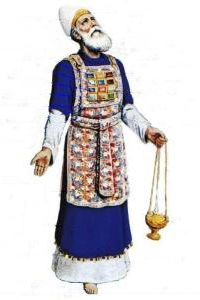
\includegraphics[width=50mm,scale=1.5]{Extras/Melchisedec.jpg}
\vspace{0.4in}  % Create a title for the document and write it in bold font
\LARGE{\textbf{\date}} % Again, do a line break
\linebreak 
% Create a subtitle \large{with Outlines, Statistics, Cross References, and Notes}
\vspace{0.5in}
\begin{flushleft}
\LARGE{Day \#75: Wednesday, 16  March 2022 PLAIN \\}\vspace{0.25in}
\LARGE{Judges 7-9 Psalm 75 Proverb 16}
\end{flushleft}
\vspace{0.6in}
\bigskip

\normalsize{Xenia, Oh.\\}
\normalsize{created: \today}
\vspace{1.3in}

\end{flushright}
\end{titlepage}

\newpage 
\tableofcontents\hypertarget{TOC}{}
\listoffigures
\listoftables

\hyphenation{A-bim-e-lech bre-thren E-phra-im  Gib-e-o-nites Jer-u-sa-lem through-out Phil-i-stines The-o-phil-us Am-a-le-kites ven-geance Mesh-el-e-mi-ah onan-ism Phar-a-oh thoughts grev-ous-ness Hach-a-liah adul-ter-er Shad-rach}

%%%%%%%%%%%%%%%%% EXTRA COLORS
%%%%%%%%%%%%%%%%% EXTRA COLORS
%%%%%%%%%%%%%%%%% EXTRA COLORS
\definecolor{champagne}{rgb}{0.97,0.91,0.81}
\definecolor{bone}{rgb}{0.89,0.85,0.79}

\definecolor{ForestGreen}{rgb}{0.00,0.29,0.098}
\definecolor{GIVING}{cmyk}{1,0.0,0.72,.1}

\definecolor{MLPE}{cmyk}{1,1,0,.45}
\definecolor{SOCCER}{cmyk}{.77, 0, .42, .49}
\definecolor{PAYBILL}{cmyk}{0,0.83,0.76,0.07}
\definecolor{SERMON}{cmyk}{.14,.9,0,.30} % aka seance \href{http://www.flatuicolorpicker.com/purple-cmyk-color-model/}{seance}
\definecolor{BIBLE}{cmyk}{0,.17,.74,.17}
\definecolor{WORKBLUE}{cmyk}{1, .5, 0, .6}
\definecolor{myOrange}{cmyk}{0, .4, .98, .03}
\definecolor{myTan}{cmyk}{0.0,.07,.17,.10}
\definecolor{myRed}{cmyk}{0,1,1,0}
\definecolor{myWhite}{cmyk}{0,0,0,0}
\definecolor{BLUESoD}{cmyk}{.97,.84,0,.04}
\definecolor{WHITE}{cmyk}{0,0,0,0}
\definecolor{OLDGOLD}{cmyk}{0.05,0.3,1.00,0}
\definecolor{CASTLETON}{cmyk}{1,0,0.31,0.66}
\definecolor{cadmiumgreen}{rgb}{0.0, 0.42, 0.24}
\definecolor{jungle}{rgb}{0.203,0.4882,0.1718}
\definecolor{MYGOLD}{rgb}{1,.84,0}

\definecolor{MYLIGHTGRAY}{rgb}{.85,.85,.85}

\definecolor{codegreen}{rgb}{0,0.6,0}
\definecolor{codegray}{rgb}{0.5,0.5,0.5}
\definecolor{codepurple}{rgb}{0.58,0,0.82}
\definecolor{backcolour}{rgb}{0.95,0.95,0.92}


\mdfdefinestyle{MyFrame}{%
    linecolor=blue,
    outerlinewidth=2pt,
    roundcorner=5pt,
    innertopmargin=\baselineskip,
    innerbottommargin=\baselineskip,
    innerrightmargin=10pt,
    innerleftmargin=10pt,
    backgroundcolor=gray!25!white}


\mdfdefinestyle{MyFrame2}{%
    linecolor=black,
    outerlinewidth=2pt,
    roundcorner=5pt,
    innertopmargin=\baselineskip,
    innerbottommargin=\baselineskip,
    innerrightmargin=10pt,
    innerleftmargin=10pt,
    backgroundcolor=yellow!25!white}


%%%%%
%% for PFTTIS list
%%%%%

%%% And Joseph said unto
\index[PFTTIS]{And Joseph said unto!Genesis!Gen 40:008}
\index[PFTTIS]{And Joseph said unto!Genesis!Gen 40:012}
\index[PFTTIS]{And Joseph said unto!Genesis!Gen 41:025}
\index[PFTTIS]{And Joseph said unto!Genesis!Gen 42:014}
\index[PFTTIS]{And Joseph said unto!Genesis!Gen 42:018}
\index[PFTTIS]{And Joseph said unto!Genesis!Gen 44:015}
\index[PFTTIS]{And Joseph said unto!Genesis!Gen 45:003}
\index[PFTTIS]{And Joseph said unto!Genesis!Gen 45:004}
\index[PFTTIS]{And Joseph said unto!Genesis!Gen 46:031}
\index[PFTTIS]{And Joseph said unto!Genesis!Gen 48:009}
\index[PFTTIS]{And Joseph said unto!Genesis!Gen 48:018}
\index[PFTTIS]{And Joseph said unto!Genesis!Gen 50:019}
\index[PFTTIS]{And Joseph said unto!Genesis!Gen 50:024}


%%% a shadow
\index[PFTTIS]{a shadow!1Chronicles!1Chr 029:15}
\index[PFTTIS]{a shadow!Job!Job 008:09}
\index[PFTTIS]{a shadow!Job!Job 014:02}
\index[PFTTIS]{a shadow!Job!Job 017:07}
\index[PFTTIS]{a shadow!Psalm!Psa 102:011}
\index[PFTTIS]{a shadow!Psalm!Psa 144:004}
\index[PFTTIS]{a shadow!Ecclesiastes!Eccl 006:012}
\index[PFTTIS]{a shadow!Ecclesiastes!Eccl 008:013}
\index[PFTTIS]{a shadow!Isaiah!Isa 04:006}
\index[PFTTIS]{a shadow!Isaiah!Isa 25:004}
\index[PFTTIS]{a shadow!Jonah!Jnh 04:06}
\index[PFTTIS]{a shadow!Colossians!Col 02:017}
\index[PFTTIS]{a shadow!Hebews!Heb 10:001}

%%% blessed is the man
\index[PFTTIS]{blessed is the man!Psalm!Psa 001:001}
\index[PFTTIS]{blessed is the man!Psalm!Psa 032:002}
\index[PFTTIS]{blessed is the man!Psalm!Psa 034:008}
\index[PFTTIS]{blessed is the man!Psalm!Psa 065:004}
\index[PFTTIS]{blessed is the man!Psalm!Psa 084:005}
\index[PFTTIS]{blessed is the man!Psalm!Psa 084:012}
\index[PFTTIS]{blessed is the man!Psalm!Psa 094:012}
\index[PFTTIS]{blessed is the man!Psalm!Psa 112:001}
\index[PFTTIS]{blessed is the man!Proverbs!Pro 008:034}
\index[PFTTIS]{blessed is the man!Isaiah!Isa 056:002}
\index[PFTTIS]{blessed is the man!Jeremiah!Jer 017:007}
\index[PFTTIS]{blessed is the man!Romans!Rom 004:008}
\index[PFTTIS]{blessed is the man!James!Jam 001:012}


%%% carry them
\index[PFTTIS]{carry them!Leviticus!Lev 14:045}
\index[PFTTIS]{carry them!Numbers!Num 11:012}
\index[PFTTIS]{carry them!Joshua!Jsh 04:003}
\index[PFTTIS]{carry them!1Samuel!1Sam 20:040}
\index[PFTTIS]{carry them!1Kings!1Kng 08:046}
\index[PFTTIS]{carry them!2Chronicles!2Chr 06:036}
\index[PFTTIS]{carry them!Ezra!Ezra 05:015}
\index[PFTTIS]{carry them!Isaiah!Isa 40:011}
\index[PFTTIS]{carry them!Isaiah!Isa 41:016}
\index[PFTTIS]{carry them!Isaiah!Isa 57:013}
\index[PFTTIS]{carry them!Jeremiah!Jer 20:004}
\index[PFTTIS]{carry them!Jeremiah!Jer 20:005}
\index[PFTTIS]{carry them!Jeremiah!Jer 43:012}


\index[PFTTIS]{good tidings!2Samuel!2Sam 18:027}
\index[PFTTIS]{good tidings!1Kings!1Ki 01:042}
\index[PFTTIS]{good tidings!2Kings!2Ki 07:009 (2x)}
\index[PFTTIS]{good tidings!Isaiah!Isa 40:009 (2x)}
\index[PFTTIS]{good tidings!Isaiah!Isa 41:007}
\index[PFTTIS]{good tidings!Isaiah!Isa 52:007}
\index[PFTTIS]{good tidings!Isaiah!Isa 61:001}
\index[PFTTIS]{good tidings!Nahum!Nah 01:005}
\index[PFTTIS]{good tidings!Luke!Lk 02:010}
\index[PFTTIS]{good tidings!1Thessalonians!1Thess 03:006}


%%% dead body
\index[PFTTIS]{dead body!Leviticus!Lev 21:011}
\index[PFTTIS]{dead body!Numbers!Num 06:006}
\index[PFTTIS]{dead body!Numbers!Num 09:006}
\index[PFTTIS]{dead body!Numbers!Num 09:007}
\index[PFTTIS]{dead body!Numbers!Num 09:010}
\index[PFTTIS]{dead body!Numbers!Num 09:011}
\index[PFTTIS]{dead body!Numbers!Num 09:013}
\index[PFTTIS]{dead body!Numbers!Num 09:016}
\index[PFTTIS]{dead body!2Kings!2Ki 08:005}
\index[PFTTIS]{dead body!Isaiah!Isa 26:019}
\index[PFTTIS]{dead body!Jeremiah!Jer 26:023}
\index[PFTTIS]{dead body!Jeremiah!Jer 36:030}
\index[PFTTIS]{dead body!Haggai!Hag 02:013}

%%% great sea
\index[PFTTIS]{great sea!Numbers!Num 34:006}
\index[PFTTIS]{great sea!Numbers!Num 34:007}
\index[PFTTIS]{great sea!Joshua!Jos 01:004}
\index[PFTTIS]{great sea!Joshua!Jos 09:001}
\index[PFTTIS]{great sea!Joshua!Jos 15:012}
\index[PFTTIS]{great sea!Joshua!Jos 15:047}
\index[PFTTIS]{great sea!Joshua!Jos 23:004}
\index[PFTTIS]{great sea!Ezekiel!Eze 47:010}
\index[PFTTIS]{great sea!Ezekiel!Eze 47:015}
\index[PFTTIS]{great sea!Ezekiel!Eze 47:019}
\index[PFTTIS]{great sea!Ezekiel!Eze 47:020}
\index[PFTTIS]{great sea!Ezekiel!Eze 48:028}
\index[PFTTIS]{great sea!Daniel!Dan 07:002}


%%% have forsaken me
\index[PFTTIS]{have forsaken me!Judges!Jdg 10:013}
\index[PFTTIS]{have forsaken me!1Samuel!1Sam 08:008}
\index[PFTTIS]{have forsaken me!1Kings!1Ki 11:033}
\index[PFTTIS]{have forsaken me!2Kings!2Ki 22:017}
\index[PFTTIS]{have forsaken me!2Chronicles!2Chr 12:005}
\index[PFTTIS]{have forsaken me!2Chronicles!2Chr 34:025}
\index[PFTTIS]{have forsaken me!Jeremiah!Jer 01:016}
\index[PFTTIS]{have forsaken me!Jeremiah!Jer 02:013}
\index[PFTTIS]{have forsaken me!Jeremiah!Jer 05:007}
\index[PFTTIS]{have forsaken me!Jeremiah!Jer 05:019}
\index[PFTTIS]{have forsaken me!Jeremiah!Jer 16:011 (2x)}
\index[PFTTIS]{have forsaken me!Jeremiah!Jer 19:004}

%%% no king
\index[PFTTIS]{no king!Judges!Jdg 17:06}
\index[PFTTIS]{no king!Judges!Jdg 18:01}
\index[PFTTIS]{no king!Judges!Jdg 19:01}
\index[PFTTIS]{no king!Judges!Jdg 21:25}
\index[PFTTIS]{no king!1Kings!1Ki 22:47}
\index[PFTTIS]{no king!2Kings!2Ki 23:25}
\index[PFTTIS]{no king!Nehemiah!Neh 13:26}
\index[PFTTIS]{no king!Psalms!Psa 033:016}
\index[PFTTIS]{no king!Proverbs!Pro 30:27}
\index[PFTTIS]{no king!Daniel!Dan 02:10}
\index[PFTTIS]{no king!Hosea!Hos 10:03}
\index[PFTTIS]{no king!Micah!Mic 04:09}
\index[PFTTIS]{no king!John!Jhn 19:15}


%%% rebellious house
\index[PFTTIS]{rebellious house!Exodus!Exo 02:005}
\index[PFTTIS]{rebellious house!Exodus!Exo 02:006}
\index[PFTTIS]{rebellious house!Exodus!Exo 02:008}
\index[PFTTIS]{rebellious house!Exodus!Exo 03:009}
\index[PFTTIS]{rebellious house!Exodus!Exo 03:026}
\index[PFTTIS]{rebellious house!Exodus!Exo 03:027}
\index[PFTTIS]{rebellious house!Exodus!Exo 12:002 (2x)}
\index[PFTTIS]{rebellious house!Exodus!Exo 12:003}
\index[PFTTIS]{rebellious house!Exodus!Exo 12:009}
\index[PFTTIS]{rebellious house!Exodus!Exo 12:025}
\index[PFTTIS]{rebellious house!Exodus!Exo 17:012}
\index[PFTTIS]{rebellious house!Exodus!Exo 24:003}

%%% seek him
\index[PFTTIS]{seek him!Deuteronomy!Deu 04:029}\index[PFTTIS]{seek him!1Samuel!1Sam 23:025}
\index[PFTTIS]{seek him!1Chronicles!1Chr 28:009}
\index[PFTTIS]{seek him!2Chronicles!1Chr 15:002}
\index[PFTTIS]{seek him!Ezra!Ezr 08:022}
\index[PFTTIS]{seek him!Psalms!Psa 022:026}
\index[PFTTIS]{seek him!Psalms!Psa 024:006}
\index[PFTTIS]{seek him!Psalms!Psa 119:002}
\index[PFTTIS]{seek him!SoS!SoS 03:002}
\index[PFTTIS]{seek him!SoS!SoS 06:001}
\index[PFTTIS]{seek him!Hosea!Hos 07:010}
\index[PFTTIS]{seek him!Amos!Amo 05:008}
\index[PFTTIS]{seek him!Hebrews!Heb 11:0063}


%%% seek ye
\index[PFTTIS]{seek ye!Isaiah!Isa 34:016}
\index[PFTTIS]{seek ye!Isaiah!Isa 45:019}
\index[PFTTIS]{seek ye!Isaiah!Isa 55:006}
\index[PFTTIS]{seek ye!Amos!Amos 5:004}
\index[PFTTIS]{seek ye!John!John 1:38}
\index[PFTTIS]{seek ye!John!John 18:4}
\index[PFTTIS]{seek ye!John!John 18:7}
\index[PFTTIS]{seek ye!Matthew!Matt 6:33}
\index[PFTTIS]{seek ye!Numbers!Num 16:10}
\index[PFTTIS]{seek ye!Luke!Luke 12:31}
\index[PFTTIS]{seek ye!Luke!Luke 24:5}
\index[PFTTIS]{seek ye!Psalm!Psa 27:8}
\index[PFTTIS]{seek ye!Zephaniah!Zeph 2:3}

%%% the uncircumcised
\index[PFTTIS]{the uncircumcised!Genesis!Gen 17:014}
\index[PFTTIS]{the uncircumcised!Judges!Jdg 14:003}
\index[PFTTIS]{the uncircumcised!Judges!Jdg 15:018}
\index[PFTTIS]{the uncircumcised!2Samuel!2Sam 01:020}
\index[PFTTIS]{the uncircumcised!Isaiah!Isa 02:001}
\index[PFTTIS]{the uncircumcised!Jeremiah!Jer 09:025}
\index[PFTTIS]{the uncircumcised!Ezekiel!Eze 28:010}
\index[PFTTIS]{the uncircumcised!Ezekiel!Eze 31:018}
\index[PFTTIS]{the uncircumcised!Ezekiel!Eze 32:019}
\index[PFTTIS]{the uncircumcised!Ezekiel!Eze 32:027}
\index[PFTTIS]{the uncircumcised!Ezekiel!Eze 32:028}
\index[PFTTIS]{the uncircumcised!Ezekiel!Eze 32:029}
\index[PFTTIS]{the uncircumcised!Ezekiel!Eze 32:032}

%%% worship him
\index[PFTTIS]{worship him!Psalms!Psa 97:007}
\index[PFTTIS]{worship him!Zephaniah!Zeph 02:011}
\index[PFTTIS]{worship him!Matthew!Matt 02:002}
\index[PFTTIS]{worship him!Matthew!Matt 02:008}
\index[PFTTIS]{worship him!John!John 04:023}
\index[PFTTIS]{worship him!John!John 04:024 (2x)} 
\index[PFTTIS]{worship him!Acts!Acts 17:023}
\index[PFTTIS]{worship him!Hebrews!Heb 01:006}
\index[PFTTIS]{worship him!Revelation!Rev 04:010}
\index[PFTTIS]{worship him!Revelation!Rev 13:008}
\index[PFTTIS]{worship him!Revelation!Rev 14:007}
\index[PFTTIS]{worship him!Revelation!Rev 19:010}


%%%%%
%% for PFTTIS list
%%%%%

%%% afflictions
\index[WFTTIS]{afflictions!Psalms!Psa 34:019}
\index[WFTTIS]{afflictions!Psalms!Psa 132:001}
\index[WFTTIS]{afflictions!Acts!Acts 07:010}
\index[WFTTIS]{afflictions!Acts!Acts 20:023}
\index[WFTTIS]{afflictions!2Corinthians!2Cor 06:004}
\index[WFTTIS]{afflictions!Colossians!Col 01:024}
\index[WFTTIS]{afflictions!1Thessalonians!1Thess 03:003}
\index[WFTTIS]{afflictions!2Timothy!2Tim 01:008}
\index[WFTTIS]{afflictions!2Timothy!2Tim 03:011}
\index[WFTTIS]{afflictions!2Timothy!2Tim 04:005}
\index[WFTTIS]{afflictions!Hebrews!Heb 10:032}
\index[WFTTIS]{afflictions!Hebrews!Heb 10:033}
\index[WFTTIS]{afflictions!1Peter!1Pet 05:009}

%%% acsend
\index[WFTTIS]{acsend!Joshua!Jos 06:05}
\index[WFTTIS]{acsend!Psalm!Psa 024:003}
\index[WFTTIS]{acsend!Psalm!Psa 135:007}
\index[WFTTIS]{acsend!Psalm!Psa 139:008}
\index[WFTTIS]{acsend!Isaiah!Isa 14:013}
\index[WFTTIS]{acsend!Isaiah!Isa 14:014}
\index[WFTTIS]{acsend!Jeremiah!Jer 10:013}
\index[WFTTIS]{acsend!Jeremiah!Jer 51:016}
\index[WFTTIS]{acsend!Ezekiel!Eze 38:009}
\index[WFTTIS]{acsend!John!John 06:062}
\index[WFTTIS]{acsend!John!John 20:017}
\index[WFTTIS]{acsend!Romans!Rom 10:006}
\index[WFTTIS]{acsend!Revelation!Rev 17:008}

%%% Assyrian
\index[WFTTIS]{Assyrian!Isaiah!Isa 10:005}
\index[WFTTIS]{Assyrian!Isaiah!Isa 10:024}
\index[WFTTIS]{Assyrian!Isaiah!Isa 14:025}
\index[WFTTIS]{Assyrian!Isaiah!Isa 19:023}
\index[WFTTIS]{Assyrian!Isaiah!Isa 23:013}
\index[WFTTIS]{Assyrian!Isaiah!Isa 30:031}
\index[WFTTIS]{Assyrian!Isaiah!Isa 31:008}
\index[WFTTIS]{Assyrian!Isaiah!Isa 52:004}
\index[WFTTIS]{Assyrian!Ezekiel!Eze 31:003}
\index[WFTTIS]{Assyrian!Hosea!Hos 05:013}
\index[WFTTIS]{Assyrian!Hosea!Hos 11:005}
\index[WFTTIS]{Assyrian!Micah!Hos 05:005}
\index[WFTTIS]{Assyrian!Micah!Hos 05:006}

%%% blot
\index[WFTTIS]{blot!Exodus!Exo 32:032}
\index[WFTTIS]{blot!Exodus!Exo 32:033}
\index[WFTTIS]{blot!Numbers!Num 05:026}
\index[WFTTIS]{blot!Deuteronomy!Deut 09:014}
\index[WFTTIS]{blot!Deuteronomy!Deut 25:019}
\index[WFTTIS]{blot!Deuteronomy!Deut 29:020}
\index[WFTTIS]{blot!2Kings!2Ki 14:027}
\index[WFTTIS]{blot!Job!Job 31:007}
\index[WFTTIS]{blot!Psalms!Psa 51:001}
\index[WFTTIS]{blot!Psalms!Psa 51:009}
\index[WFTTIS]{blot!Proverbs!Pro 09:007}
\index[WFTTIS]{blot!Jeremiah!Jer 18:023}
\index[WFTTIS]{blot!Revelation!Rev 03:005}


%%% chain
\index[WFTTIS]{chain!Genesis!Gen 41:042}
\index[WFTTIS]{chain!1Kings!1Ki 07:017}
\index[WFTTIS]{chain!Psalms!Psa 73:006}
\index[WFTTIS]{chain!SoS!Sos 04:009}
\index[WFTTIS]{chain!Lamentations!Lam 03:007}
\index[WFTTIS]{chain!Ezekiel!Eze 07:023}
\index[WFTTIS]{chain!Ezekiel!Eze 16:011}
\index[WFTTIS]{chain!Daniel!Dan 05:007}
\index[WFTTIS]{chain!Daniel!Dan 05:016}
\index[WFTTIS]{chain!Daniel!Dan 05:029}
\index[WFTTIS]{chain!Acts!Acts 28:020}
\index[WFTTIS]{chain!2Timothy!2Tim 01:016}
\index[WFTTIS]{chain!Revelation!Rev 20:001}


%%% controversy
\index[WFTTIS]{controversy!Deuteronomy!Deu 17:008}
\index[WFTTIS]{controversy!Deuteronomy!Deu 19:017}
\index[WFTTIS]{controversy!Deuteronomy!Deu 21:005}
\index[WFTTIS]{controversy!Deuteronomy!Deu 25:001}
\index[WFTTIS]{controversy!2Samuel!2Sam 15:002}
\index[WFTTIS]{controversy!Isaiah!Isa 34:008}
\index[WFTTIS]{controversy!Jeremiah!Jer 25:031}
\index[WFTTIS]{controversy!Ezekiel!Eze 44:024}
\index[WFTTIS]{controversy!Hosea!Hos 04:001}
\index[WFTTIS]{controversy!Hosea!Hos 12:002}
\index[WFTTIS]{controversy!Micah!Mic 06:002 (2x)}
\index[WFTTIS]{controversy!1Timothy!1Tim 03:016}


%%% Dagon/Dagon's
\index[WFTTIS]{Dagon!Judges!Jdg 16:023}
\index[WFTTIS]{Dagon!1Samuel!1Sam 05:002 (2x)}
\index[WFTTIS]{Dagon!1Samuel!1Sam 05:003 (2x)}
\index[WFTTIS]{Dagon!1Samuel!1Sam 05:004 (3x)}
\index[WFTTIS]{Dagon!1Samuel!1Sam 05:005 (3x)}
\index[WFTTIS]{Dagon!1Samuel!1Sam 05:007}
\index[WFTTIS]{Dagon!1Chronicles!1Chr 10:010}

%%% disobedient
\index[WFTTIS]{disobedient!1Kings!1Ki 13:026}
\index[WFTTIS]{disobedient!Nehemiah!Neh 09:026}
\index[WFTTIS]{disobedient!Luke!Luke 01:017}
\index[WFTTIS]{disobedient!Acts!Acts 26:019}
\index[WFTTIS]{disobedient!Romans!Rom 01:030}
\index[WFTTIS]{disobedient!Romans!Rom 10:021}
\index[WFTTIS]{disobedient!1Timothy!1Tim 01:009}
\index[WFTTIS]{disobedient!2Timothy!2Tim 03:002}
\index[WFTTIS]{disobedient!Titus!Titus 01:016}
\index[WFTTIS]{disobedient!Titus!Titus 03:003}
\index[WFTTIS]{disobedient!1Peter!1Pet 02:007}
\index[WFTTIS]{disobedient!1Peter!1Pet 02:008}
\index[WFTTIS]{disobedient!1Peter!1Pet 03:020}


%%% doubt
\index[WFTTIS]{doubt!Genesis!Gen 37:033}
\index[WFTTIS]{doubt!Deuteronomy!Deu 28:066}
\index[WFTTIS]{doubt!Job!Job 12:002}
\index[WFTTIS]{doubt!Matthew!Matt 14:031}
\index[WFTTIS]{doubt!Matthew!Matt 21:021}
\index[WFTTIS]{doubt!Mark!Mk 11:023}
\index[WFTTIS]{doubt!Luke!Lk 11:020}
\index[WFTTIS]{doubt!John!Jhn 10:024}
\index[WFTTIS]{doubt!Acts!Acts 02:012}
\index[WFTTIS]{doubt!Acts!Acts 28:004}
\index[WFTTIS]{doubt!1Corinthians!1Cor 09:010}
\index[WFTTIS]{doubt!Galatians!Gal 04:020}
\index[WFTTIS]{doubt!1John!1Jhn 02:019}


%%% dungeon
\index[WFTTIS]{dungeon!Genesis!Gen 40:015}
\index[WFTTIS]{dungeon!Genesis!Gen 41:014}
\index[WFTTIS]{dungeon!Exodus!Exo 12:029}
\index[WFTTIS]{dungeon!Jeremiah!Jer 37:016}
\index[WFTTIS]{dungeon!Jeremiah!Jer 38:006 (2x)}
\index[WFTTIS]{dungeon!Jeremiah!Jer 38:007}
\index[WFTTIS]{dungeon!Jeremiah!Jer 38:009}
\index[WFTTIS]{dungeon!Jeremiah!Jer 38:010}
\index[WFTTIS]{dungeon!Jeremiah!Jer 38:011}
\index[WFTTIS]{dungeon!Jeremiah!Jer 38:013}
\index[WFTTIS]{dungeon!Lamentations!Lam 03:053}
\index[WFTTIS]{dungeon!Lamentations!Lam 03:055}


%%% error
\index[WFTTIS]{error!2Samuel!2Sam 06:007}
\index[WFTTIS]{error!Job!Job 19:004}
\index[WFTTIS]{error!Ecclesiastes!Ecc 05:006}
\index[WFTTIS]{error!Ecclesiastes!Ecc 10:005}
\index[WFTTIS]{error!Isaiah!Isa 32:006}
\index[WFTTIS]{error!Daniel!Dan 06:004}
\index[WFTTIS]{error!Matthew!Matt 27:064}
\index[WFTTIS]{error!Romans!Rom 01:027}
\index[WFTTIS]{error!James!Jam 05:020}
\index[WFTTIS]{error!2Peter!2Pet 02:018}
\index[WFTTIS]{error!2Peter!2Pet 03:017}
\index[WFTTIS]{error!1John!1Jn 04:006}
\index[WFTTIS]{error!Jude!Jude 01:011}

%%% fourish
\index[WFTTIS]{fourish!Psalms!Psa 072:007}
\index[WFTTIS]{fourish!Psalms!Psa 072:016}
\index[WFTTIS]{fourish!Psalms!Psa 092:007}
\index[WFTTIS]{fourish!Psalms!Psa 092:012}
\index[WFTTIS]{fourish!Psalms!Psa 092:013}
\index[WFTTIS]{fourish!Psalms!Psa 132:018}
\index[WFTTIS]{fourish!Proverbs!Pro 11:28}
\index[WFTTIS]{fourish!Proverbs!Pro 14:11}
\index[WFTTIS]{fourish!Ecclesiastes!Ecc 12:05}
\index[WFTTIS]{fourish!SongOfSolomon!SOS 07:12}
\index[WFTTIS]{fourish!Isaiah!Isa 17:11}
\index[WFTTIS]{fourish!Isaiah!Isa 66:14}
\index[WFTTIS]{fourish!Ezekiel!Eze 17:24}




%%% giants
\index[WFTTIS]{giants!Genesis!Gen 06:004}
\index[WFTTIS]{giants!Numbers!Num 13:033}
\index[WFTTIS]{giants!Deuteronomy!Deut 02:011}
\index[WFTTIS]{giants!Deuteronomy!Deut 02:021}
\index[WFTTIS]{giants!Deuteronomy!Deut 03:011}
\index[WFTTIS]{giants!Deuteronomy!Deut 03:013}
\index[WFTTIS]{giants!Joshua!Josh 12:004}
\index[WFTTIS]{giants!Joshua!Josh 13:012}
\index[WFTTIS]{giants!Joshua!Josh 15:008}
\index[WFTTIS]{giants!Joshua!Josh 17:015}
\index[WFTTIS]{giants!Joshua!Josh 16:016}

%%% good man
\index[WFTTIS]{good man!2 Samuel!2Sa 18:27}
%(1) Psalms 37:23 [5]
%(1) Psalms 112:5 [2]
%(1) Proverbs 12:2 [2]
%(1) Proverbs 13:22 [2]
%(1) Proverbs 14:14 [14]
%(1) Micah 7:2 [2]
%(1) Matthew 12:35 [2]
%(1) Luke 6:45 [2]
%(1) Luke 23:50 [15]
%(1) John 7:12 [17]
%(1) Acts 11:24 [5]
%(1) Romans 5:7 [14]

%%% Hinnom
\index[WFTTIS]{Hinnom!Joshua!Jsh 15:008}
\index[WFTTIS]{Hinnom!Joshua!Jsh 18:016}
\index[WFTTIS]{Hinnom!2Kings!2Ki 23:010}
\index[WFTTIS]{Hinnom!2Chronicles!2Chr 28:003}
\index[WFTTIS]{Hinnom!2Chronicles!2Chr 33:006}
\index[WFTTIS]{Hinnom!Nehemiah!Neh 11:030}
\index[WFTTIS]{Hinnom!Jeremiah!Jer 07:031}
\index[WFTTIS]{Hinnom!Jeremiah!Jer 07:032}
\index[WFTTIS]{Hinnom!Jeremiah!Jer 19:002}
\index[WFTTIS]{Hinnom!Jeremiah!Jer 19:006}
\index[WFTTIS]{Hinnom!Jeremiah!Jer 32:035}

%%% inclined
\index[WFTTIS]{inclined!Judges!Jdg 09:003}
\index[WFTTIS]{inclined!Psalms!Psa 040:001}
\index[WFTTIS]{inclined!Psalms!Psa 116:002}
\index[WFTTIS]{inclined!Psalms!Psa 119:112}
\index[WFTTIS]{inclined!Proverbs!Pro 05:13}
\index[WFTTIS]{inclined!Jeremiah!Jer 07:24}
\index[WFTTIS]{inclined!Jeremiah!Jer 07:26}
\index[WFTTIS]{inclined!Jeremiah!Jer 11:08}
\index[WFTTIS]{inclined!Jeremiah!Jer 17:23}
\index[WFTTIS]{inclined!Jeremiah!Jer 25:04}
\index[WFTTIS]{inclined!Jeremiah!Jer 34:14}
\index[WFTTIS]{inclined!Jeremiah!Jer 35:15}
\index[WFTTIS]{inclined!Jeremiah!Jer 44:05}


%%% laughed
\index[WFTTIS]{laughed!Genesis!Gen 17:017}
\index[WFTTIS]{laughed!Genesis!Gen 18:012}
\index[WFTTIS]{laughed!Genesis!Gen 18:015}
\index[WFTTIS]{laughed!2Kings!2Ki 19:021}
\index[WFTTIS]{laughed!2Chronicles!2Chr 30:010}
\index[WFTTIS]{laughed!Nehemiah!Neh 02:019}
\index[WFTTIS]{laughed!Job!Job 12:004}
\index[WFTTIS]{laughed!Job!Job 29:024}
\index[WFTTIS]{laughed!Isaiah!Isa 37:022}
\index[WFTTIS]{laughed!Ezekiel!Ezek 23:032}
\index[WFTTIS]{laughed!Matthew!Matt 09:024}
\index[WFTTIS]{laughed!Mark!Mk 05:040}
\index[WFTTIS]{laughed!Luke!Lk 08:053}

%%% liar
\index[WFTTIS]{liar!Job!Job 24:025}
\index[WFTTIS]{liar!Proverbs!Pro 17:004}
\index[WFTTIS]{liar!Proverbs!Pro 19:022}
\index[WFTTIS]{liar!Proverbs!Pro 30:006}
\index[WFTTIS]{liar!Jeremiah!Jer 15:018}
\index[WFTTIS]{liar!John!Jhn 08:044}
\index[WFTTIS]{liar!John!Jhn 08:055}
\index[WFTTIS]{liar!Romans!Rom 03:004}
\index[WFTTIS]{liar!1John!1Jhn 01:010}
\index[WFTTIS]{liar!1John!1Jhn 02:004}
\index[WFTTIS]{liar!1John!1Jhn 02:022}
\index[WFTTIS]{liar!1John!1Jhn 04:020}
\index[WFTTIS]{liar!1John!1Jhn 05:010}

%%% palsy
\index[WFTTIS]{palsy!Matthew!Matt 04:024}
\index[WFTTIS]{palsy!Matthew!Matt 08:006}
\index[WFTTIS]{palsy!Matthew!Matt 09:002}
\index[WFTTIS]{palsy!Matthew!Matt 09:006}
\index[WFTTIS]{palsy!Mark!Mk 02:003}
\index[WFTTIS]{palsy!Mark!Mk 02:004}
\index[WFTTIS]{palsy!Mark!Mk 02:005}
\index[WFTTIS]{palsy!Mark!Mk 02:009}
\index[WFTTIS]{palsy!Mark!Mk 02:010}
\index[WFTTIS]{palsy!Luke!Lk 05:018}
\index[WFTTIS]{palsy!Luke!Lk 05:024}
\index[WFTTIS]{palsy!Acts!Acts 09:033}

%%% Profitable
\index[WFTTIS]{profitable!Job!Job 22:002 (2x)}
\index[WFTTIS]{profitable!Ecclesiastes!Ecc 10:010}
\index[WFTTIS]{profitable!Isaiah!Isa 44:010}
\index[WFTTIS]{profitable!Jeremiah!Jer 13:007}
\index[WFTTIS]{profitable!Matthew!Matt 05:029}
\index[WFTTIS]{profitable!Matthew!Matt 05:030}
\index[WFTTIS]{profitable!Acts!Acts 20:020}
\index[WFTTIS]{profitable!1Timothy!1Tim 04:008}
\index[WFTTIS]{profitable!2Timothy!2Tim 03:016}
\index[WFTTIS]{profitable!2Timothy!2Tim 04:011}
\index[WFTTIS]{profitable!Titus!Titus 03:008}
\index[WFTTIS]{profitable!Philemon!Phlm 01:011}

%%% Rechab
\index[WFTTIS]{Rechab!2Samuel!2Sam 04:002}
\index[WFTTIS]{Rechab!2Samuel!2Sam 04:005}
\index[WFTTIS]{Rechab!2Samuel!2Sam 04:006}
\index[WFTTIS]{Rechab!2Samuel!2Sam 04:009}
\index[WFTTIS]{Rechab!2KIngs!2Ki 10:015}
\index[WFTTIS]{Rechab!2KIngs!2Ki 10:023}
\index[WFTTIS]{Rechab!1Chronicles!1Chr 02:055}
\index[WFTTIS]{Rechab!Nehemiah!Neh 03:014}
\index[WFTTIS]{Rechab!Jeremiah!Jer 35:006}
\index[WFTTIS]{Rechab!Jeremiah!Jer 35:008}
\index[WFTTIS]{Rechab!Jeremiah!Jer 35:014}
\index[WFTTIS]{Rechab!Jeremiah!Jer 35:016}
\index[WFTTIS]{Rechab!Jeremiah!Jer 35:019}

%%% serpents
\index[WFTTIS]{serpents!Exodus!Exo 07:012}
\index[WFTTIS]{serpents!Numbers!Num 21:006}
\index[WFTTIS]{serpents!Numbers!Num 21:007}
\index[WFTTIS]{serpents!Deuteronomy!Deu 08:015}
\index[WFTTIS]{serpents!Deuteronomy!Deu 32:024}
\index[WFTTIS]{serpents!Jeremiah!Jer 08:017}
\index[WFTTIS]{serpents!Matthew!Matt 10:016}
\index[WFTTIS]{serpents!Matthew!Matt 23:033}
\index[WFTTIS]{serpents!Mark!Mk 16:018}
\index[WFTTIS]{serpents!Luke!Lk 10:019}
\index[WFTTIS]{serpents!1Corinthians!1Cor 10:009}
\index[WFTTIS]{serpents!James!Jas 03:007}
\index[WFTTIS]{serpents!Revelation!Rev 09:019}

%%% short
\index[WFTTIS]{short!Numbers!Num 11:023}
\index[WFTTIS]{short!2Kings!2Ki 10:032}
\index[WFTTIS]{short!Job!Job 17:012}
\index[WFTTIS]{short!Job!Job 20:005}
\index[WFTTIS]{short!Psalms!Psa 89:047}
\index[WFTTIS]{short!Romans!Rom 03:023}
\index[WFTTIS]{short!Romans!Rom 09:028  (2x)}
\index[WFTTIS]{short!1Corinthians!1Cor 07:029}
\index[WFTTIS]{short!1Thessalonians!1Thess 02:017}
\index[WFTTIS]{short!Hebrews!Heb 04:001}
\index[WFTTIS]{short!Revelation!Rev 12:012}
\index[WFTTIS]{short!Revelation!Rev 17:010}

%%% smiteth
\index[WFTTIS]{smiteth!Exodus!Exo 21:012}
\index[WFTTIS]{smiteth!Exodus!Exo 21:15}
\index[WFTTIS]{smiteth!Deuteronomy!Dt 25:11}
\index[WFTTIS]{smiteth!Deuteronomy!Dt 27:24}
\index[WFTTIS]{smiteth!Joshua!Jsh 15:16}
\index[WFTTIS]{smiteth!Judges!Jdg 15:16}
\index[WFTTIS]{smiteth!2 Samuel!2Sa 05:08}
\index[WFTTIS]{smiteth!1Chronicles!1Chr 11:06}
\index[WFTTIS]{smiteth!Job!1Chr 26:12}
\index[WFTTIS]{smiteth!Isaiah!Isa 09:13}
\index[WFTTIS]{smiteth!Lamentations!Lam 03:30}
\index[WFTTIS]{smiteth!Ezekiel!Eze 07:09}
\index[WFTTIS]{smiteth!Luke!Lk 06:29}



%%% vanities
\index[WFTTIS]{vanities!Deuteronomy!Deut 21:021}
\index[WFTTIS]{vanities!1Kings!1Ki 16:013}
\index[WFTTIS]{vanities!1Kings!1Ki 16:026}
\index[WFTTIS]{vanities!Psalms!Psa 031:006}
\index[WFTTIS]{vanities!Ecclesiastes!Ecc 01:002 (2x)}
\index[WFTTIS]{vanities!Ecclesiastes!Ecc 05:007}
\index[WFTTIS]{vanities!Ecclesiastes!Ecc 12:008}
\index[WFTTIS]{vanities!Jeremiah!Jer 08:019}
\index[WFTTIS]{vanities!Jeremiah!Jer 10:008}
\index[WFTTIS]{vanities!Jeremiah!Jer 14:022}
\index[WFTTIS]{vanities!Jonah!Jnh 02:008}
\index[WFTTIS]{vanities!Acts!Acts 14:015}



%%%%%
%% for PFTTIS list
%%%%%

%%% worm
\index[WFITV]{worm!Exodus!Exo 16:024}
\index[WFITV]{worm!Job!Job 17:014}
\index[WFITV]{worm!Job!Job 24:029}
\index[WFITV]{worm!Job!Job 25:005 (2x)}
\index[WFITV]{worm!Psalms!Psa 022:006}
\index[WFITV]{worm!Isaiah!Isa 14:011}
\index[WFITV]{worm!Isaiah!Isa 41:014}
\index[WFITV]{worm!Isaiah!Isa 51:008}
\index[WFITV]{worm!Isaiah!Isa 66:024}
\index[WFITV]{worm!Jonah!Jnh 04:007}
\index[WFITV]{worm!Mark!Mk 09:044}
\index[WFITV]{worm!Mark!Mk 09:046}
\index[WFITV]{worm!Mark!Mk 09:048}


%\subsubsection{Title}
%\textbf{Introduction:} Isaiah 46 
%\index[speaker]{Speaker!Isaiah 49 (Title}
%\index[series]{Book (Speaker)!IPassage (Title)}
%\index[date]{2017/07/09!Isaiah 49 (Title)}
%\begin{compactenum}[I.]
%    \item  \textbf{Point} \index[scripture]{Isaiah!IPassage} (IPassage)
%\end{compactenum}




  

\chapter{Judges 7}

\begin{figure}
  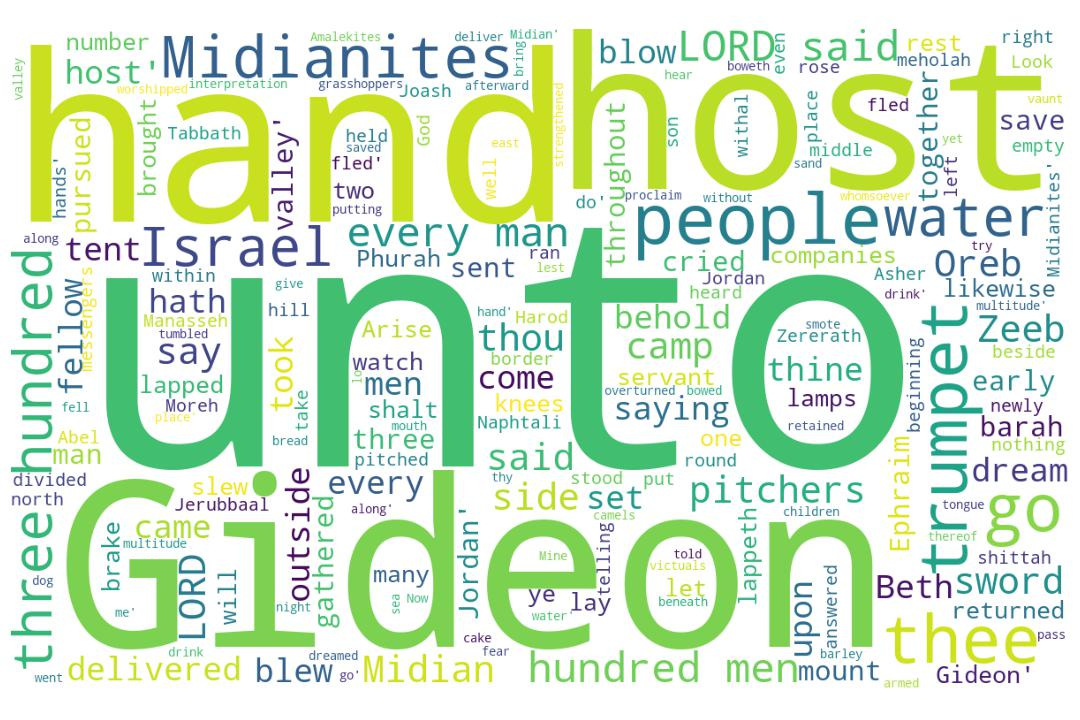
\includegraphics[width=\linewidth]{07OT-Judges/Judges7-WordCloud.jpg}
  \caption{Judges 7 Word Cloud}
  \label{fig:Judges 7 Word Cloud}
\end{figure}


\marginpar{\scriptsize \centering \fcolorbox{bone}{lime}{\textbf{GOD CHOOSES}}\\ (Judges 7) \begin{compactenum}[I.][8]
    \item The \textbf{Mount} \index[scripture]{Judges!Judges 07:03}(Jdg 7:3)
    \item The \textbf{Remiaining} Ones \index[scripture]{Judges!Judges 07:03}(Jdg 7:3)
    \item Those who were \textbf{Mindful} \index[scripture]{Judges!Judges 07:06}(Jdg 7:6)
    \item The Host of \textbf{Midian} \index[scripture]{Judges!Judges 07:08}(Jdg 7:8)
    \item Like Grasshopper for  \textbf{Multitude} \index[scripture]{Judges!Judges 07:12}(Jdg 7:12)
    \item The  \textbf{Music} \index[scripture]{Judges!Judges 07:12}(Jdg 7:12)
    \item Sent \textbf{Messengers} \index[scripture]{Judges!Judges 07:24}(Jdg 7:24)
\end{compactenum}}

\marginpar{\scriptsize \centering \fcolorbox{bone}{yellow}{\textbf{HEARTS \& MINDS}}\\ (Judges 7) \begin{compactenum}[I.][8]
    \item The \textbf{People} \index[scripture]{Judges!Judges 07:01}\index[scripture]{Judges!Judges 07:02}\index[scripture]{Judges!Judges 07:03}\index[scripture]{Judges!Judges 07:04}\index[scripture]{Judges!Judges 07:05}\index[scripture]{Judges!Judges 07:06}\index[scripture]{Judges!Judges 07:07}\index[scripture]{Judges!Judges 07:08}
    (Jdg 7:1, 2, 3, 4, 5, 6, 7, 8)
    \item The \textbf{Proclamation} \index[scripture]{Judges!Judges 07:03}(Jdg 7:3)
    \item \textbf{Pruning} \index[scripture]{Judges!Judges 07:06}(Jdg 7:6)
	\item \textbf{Phurah} \index[scripture]{Judges!Judges 07:11} \index[scripture]{Judges!Judges 07:12}(Jdg 7:11, 12)
    \item The \textbf{Perception} of the Enemy \index[scripture]{Judges!Judges 07:13-14}(Jdg 7:13-14)
    \item The \textbf{Placement} \index[scripture]{Judges!Judges 07:16}(Jdg 7:16)
    \item The \textbf{Plan} \index[scripture]{Judges!Judges 07:18}(Jdg 7:18)
\end{compactenum}}

\marginpar{\scriptsize \centering \fcolorbox{bone}{black}{\textbf{\textcolor[cmyk]{0,0,0,0}{MYSTERIOUS WAYS}}}\\ (Judges 7) 
\begin{compactenum}[I.][8]
    \item Defy \textbf{Explanation} %\index[scripture]{Judges!Judges 07:04}(Jdg 7:4)
    \item Defy \textbf{Expression} %\index[scripture]{Judges!Judges 07:04}(Jdg 7:4)
    \item Defy \textbf{Experience} %\index[scripture]{Judges!Judges 07:04}(Jdg 7:4)
    \item Defy \textbf{Evidence} %\index[scripture]{Judges!Judges 07:04}(Jdg 7:4)
    \item Defy \textbf{Exception} %\index[scripture]{Judges!Judges 07:04}(Jdg 7:4)
    \item Defy \textbf{Expedience} %\index[scripture]{Judges!Judges 07:04}(Jdg 7:4)
    \item Defy \textbf{Examination} %\index[scripture]{Judges!Judges 07:04}(Jdg 7:4)
\end{compactenum}}

\footnote{\textcolor[rgb]{0.00,0.25,0.00}{\hyperlink{JudgesTOC}{Return to end of Table of Contents.}}}\footnote{\href{https://audiobible.com/bible/judges_7.html}{\textcolor[cmyk]{0.99998,1,0,0}{Judges 7 Audio}}}\textcolor[cmyk]{0.99998,1,0,0}{Then Jerubbaal, who \emph{is} \fcolorbox{bone}{bone}{Gideon}, and \fcolorbox{bone}{bone}{all} the people that \emph{were} with him, rose up early, and pitched beside the well of Harod: so that \fcolorbox{bone}{bone}{the host} of the Midianites were on the north side of them, by the hill of Moreh, \fcolorbox{bone}{bone}{in} the valley.}
[2] \textcolor[cmyk]{0.99998,1,0,0}{And the LORD said unto \fcolorbox{bone}{bone}{Gideon}, The people that \emph{are} with thee \emph{are} too many for me to give the Midianites into their hands, lest Israel vaunt themselves against me, saying, Mine own hand hath saved me.}
[3] \textcolor[cmyk]{0.99998,1,0,0}{Now therefore go to, proclaim \fcolorbox{bone}{bone}{in} the ears of the people, saying, Whosoever \emph{is} fearful and afraid, let him return and depart early from \fcolorbox{bone}{lime}{mount} Gilead. And there returned of the people twenty and two thousand; and there \fcolorbox{bone}{lime}{remained} ten thousand.}
[4] \textcolor[cmyk]{0.99998,1,0,0}{And the LORD said unto \fcolorbox{bone}{bone}{Gideon}, The people \emph{are} yet \emph{too} many; bring them down unto the water, and I will try them for thee there: and it shall be, \emph{that} of whom I say unto thee, This shall go with thee, the same shall go with thee; and of whomsoever I say unto thee, This shall not go with thee, the same shall not go.}
[5] \textcolor[cmyk]{0.99998,1,0,0}{So he brought down the people unto the water: and the LORD said unto \fcolorbox{bone}{bone}{Gideon}, Every one that lappeth of the water with his tongue, as a dog lappeth, him shalt thou set by himself; likewise every one that boweth down upon his knees to drink.}
[6] \textcolor[cmyk]{0.99998,1,0,0}{And the number of \fcolorbox{bone}{lime}{them that lapped}, \emph{putting} their hand to their mouth, were three hundred men: but \fcolorbox{bone}{bone}{all} the rest of the people bowed down upon their knees to drink water.}
[7] \textcolor[cmyk]{0.99998,1,0,0}{And the LORD said unto \fcolorbox{bone}{bone}{Gideon}, By the three hundred men that lapped will I save you, and deliver the Midianites into thine hand: and let \fcolorbox{bone}{bone}{all} the \emph{other} people go every man unto his place.}
[8] \textcolor[cmyk]{0.99998,1,0,0}{So the people took victuals \fcolorbox{bone}{bone}{in} their hand, and their trumpets: and he sent \fcolorbox{bone}{bone}{all} \emph{the} \emph{rest} \emph{of} Israel every man unto his tent, and retained those three hundred men: and \fcolorbox{bone}{bone}{the host} of \fcolorbox{bone}{lime}{Midian} was beneath him \fcolorbox{bone}{bone}{in} the valley.}\\
\\
\P \textcolor[cmyk]{0.99998,1,0,0}{And it came to pass the same night, that the LORD said unto him, Arise, get thee down unto \fcolorbox{bone}{bone}{the host}; for I have delivered it into thine hand.}
[10] \textcolor[cmyk]{0.99998,1,0,0}{But if thou fear to go down, go thou with Phurah thy servant down to \fcolorbox{bone}{bone}{the host}:}
[11] \textcolor[cmyk]{0.99998,1,0,0}{And thou shalt hear what they say; and afterward shall thine hands be strengthened to go down unto \fcolorbox{bone}{bone}{the host}. Then went he down with Phurah his servant unto the outside of the armed men that \emph{were} \fcolorbox{bone}{bone}{in} \fcolorbox{bone}{bone}{the host}.}
[12] \textcolor[cmyk]{0.99998,1,0,0}{And the Midianites and the Amalekites and \fcolorbox{bone}{bone}{all} the children of the east lay along \fcolorbox{bone}{bone}{in} the valley like \fcolorbox{bone}{lime}{grasshoppers for multitude}; and their camels \emph{were} without number, as the sand by the sea side for multitude.}
[13] \textcolor[cmyk]{0.99998,1,0,0}{And when \fcolorbox{bone}{bone}{Gideon} was come, behold, \emph{there} \emph{was} a man that told a dream unto his fellow, and said, Behold, I dreamed a dream, and, lo, a cake of barley bread tumbled into \fcolorbox{bone}{bone}{the host} of Midian, and came unto a tent, and smote it that it fell, and overturned it, that the tent lay along.}
[14] \textcolor[cmyk]{0.99998,1,0,0}{And his fellow answered and said, This \emph{is} nothing else save the sword of \fcolorbox{bone}{bone}{Gideon} the son of Joash, a man of Israel: \emph{for} into his hand hath God delivered Midian, and \fcolorbox{bone}{bone}{all} \fcolorbox{bone}{bone}{the host}.}\\
\\
\P \textcolor[cmyk]{0.99998,1,0,0}{And it was \emph{so}, when \fcolorbox{bone}{bone}{Gideon} heard the telling of the dream, and the interpretation thereof, that he worshipped, and returned into \fcolorbox{bone}{bone}{the host} of Israel, and said, Arise; for the LORD hath delivered into your hand \fcolorbox{bone}{bone}{the host} of Midian.}
[16] \textcolor[cmyk]{0.99998,1,0,0}{And he divided the three hundred men \emph{into} three companies, and he put a trumpet \fcolorbox{bone}{bone}{in} every man's hand, with empty pitchers, and lamps within the pitchers.}
[17] \textcolor[cmyk]{0.99998,1,0,0}{And he said unto them, Look on me, and do likewise: and, behold, when I come to the outside of the camp, it shall be \emph{that}, as I do, so shall ye do.}
[18] \textcolor[cmyk]{0.99998,1,0,0}{When I blow with a trumpet, I and \fcolorbox{bone}{bone}{all} that \emph{are} with me, then blow ye the trumpets also on every side of \fcolorbox{bone}{bone}{all} the camp, and say, \emph{The} \emph{sword} of the LORD, and of \fcolorbox{bone}{bone}{Gideon}.}\\
\\
\P \textcolor[cmyk]{0.99998,1,0,0}{So \fcolorbox{bone}{bone}{Gideon}, and the hundred men that \emph{were} with him, came unto the outside of the camp \fcolorbox{bone}{bone}{in} the beginning of the middle watch; and they had but newly set the watch: and they blew the \fcolorbox{bone}{lime}{trumpets}, and brake the pitchers that \emph{were} \fcolorbox{bone}{bone}{in} their hands.}
[20] \textcolor[cmyk]{0.99998,1,0,0}{And the three companies blew the trumpets, and brake the pitchers, and held the lamps \fcolorbox{bone}{bone}{in} their left hands, and the trumpets \fcolorbox{bone}{bone}{in} their right hands to blow \emph{withal}: and they cried, The sword of the LORD, and of \fcolorbox{bone}{bone}{Gideon}.}
[21] \textcolor[cmyk]{0.99998,1,0,0}{And they stood every man \fcolorbox{bone}{bone}{in} his place round about the camp: and \fcolorbox{bone}{bone}{all} \fcolorbox{bone}{bone}{the host} ran, and cried, and fled.}
[22] \textcolor[cmyk]{0.99998,1,0,0}{And the three hundred blew the trumpets, and the LORD set every man's sword against his fellow, even throughout \fcolorbox{bone}{bone}{all} \fcolorbox{bone}{bone}{the host}: and \fcolorbox{bone}{bone}{the host} fled to Beth-shittah \fcolorbox{bone}{bone}{in} Zererath, \emph{and} to the border of Abel-meholah, unto Tabbath.}
[23] \textcolor[cmyk]{0.99998,1,0,0}{And the men of Israel gathered themselves together out of Naphtali, and out of Asher, and out of \fcolorbox{bone}{bone}{all} Manasseh, and pursued after the Midianites.}\\
\\
\P \textcolor[cmyk]{0.99998,1,0,0}{And \fcolorbox{bone}{bone}{Gideon} sent \fcolorbox{bone}{lime}{messengers} throughout \fcolorbox{bone}{bone}{all} mount Ephraim, saying, Come down against the Midianites, and take before them the waters unto Beth-barah and Jordan. Then \fcolorbox{bone}{bone}{all} the men of Ephraim gathered themselves together, and took the waters unto Beth-barah and Jordan.}
[25] \textcolor[cmyk]{0.99998,1,0,0}{And they took two princes of the Midianites, Oreb and Zeeb; and they slew Oreb upon the rock Oreb, and Zeeb they slew at the winepress of Zeeb, and pursued Midian, and brought the heads of Oreb and Zeeb to \fcolorbox{bone}{bone}{Gideon} on the other side Jordan.}
\chapter{Judges 8}
 
\begin{figure}
  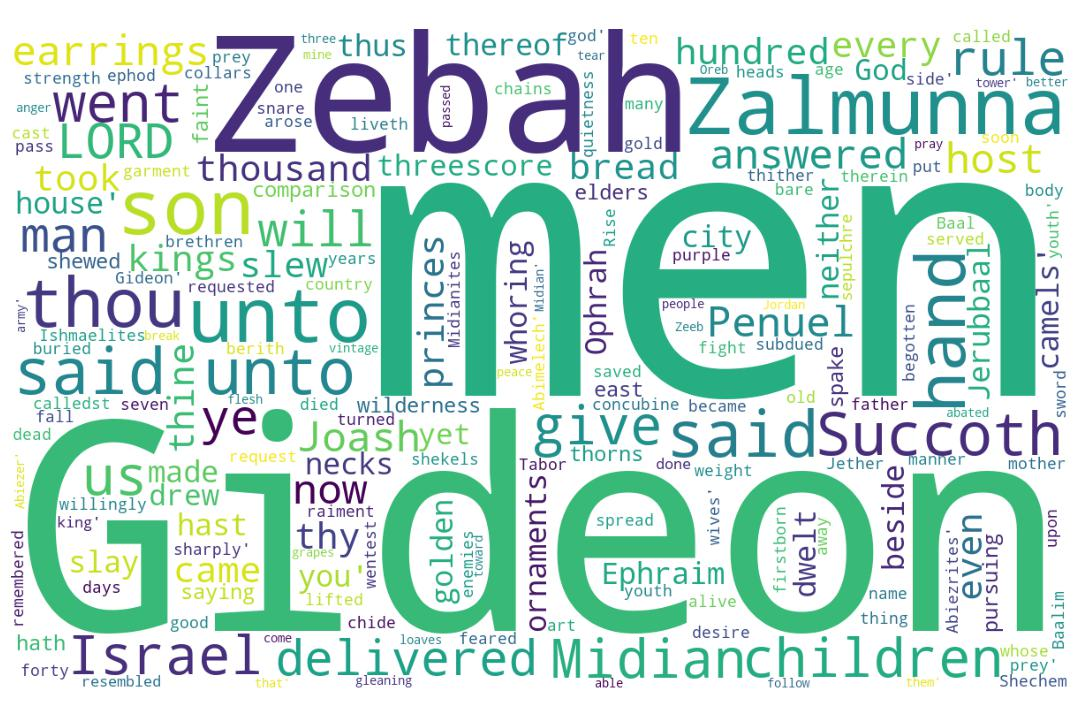
\includegraphics[width=\linewidth]{07OT-Judges/Judges8-WordCloud.jpg}
  \caption{Judges 8 Word Cloud}
  \label{fig:Judges 8 Word Cloud}
\end{figure}


\marginpar{\scriptsize \centering \fcolorbox{bone}{lime}{\textbf{GIDEON'S FAME}}\\ (Judges 8) \begin{compactenum}[I.][8]
    \item \textbf{Made a Hero} \index[scripture]{Judges!Judges 08:12}(Jdg 8:12)
    \item \textbf{Mostly Right} %\index[scripture]{Judges!Judges 07:04}(Judges 7:4)
    \item \textbf{Morally Suspect} \index[scripture]{Judges!Judges 08:24}(Jdg 8:24)
    \item \textbf{Mistreated by the Brethren} \index[scripture]{Judges!Judges 08:06, 08}(Jdg 8:6, 8)
    \item \textbf{Remembered no More} \index[scripture]{Judges!Judges 08:35}(Jdg 8:35)
    \item \textbf{Might in the Flesh} \index[scripture]{Judges!Judges 08:30}(Jdg 8:30)
    \item A \textbf{Momentary Hero} \index[scripture]{Judges!Judges 08:35}(Jdg 8:35)
\end{compactenum}}


\footnote{\textcolor[rgb]{0.00,0.25,0.00}{\hyperlink{JudgesTOC}{Return to end of Table of Contents.}}}\footnote{\href{https://audiobible.com/bible/judges_7.html}{\textcolor[cmyk]{0.99998,1,0,0}{Judges 7 Audio}}}\textcolor[cmyk]{0.99998,1,0,0}{And the men of Ephraim said unto him, Why hast thou served us thus, that thou calledst us not, when thou wentest to fight with the Midianites? And they did chide with him sharply.}
[2] \textcolor[cmyk]{0.99998,1,0,0}{And he said unto them, What have I done now in comparison of you? \emph{Is} not the gleaning of the grapes of Ephraim better than the vintage of Abiezer?}
[3] \textcolor[cmyk]{0.99998,1,0,0}{God hath delivered into your hands the princes of Midian, Oreb and Zeeb: and what was I able to do in comparison of you? Then their anger was abated toward him, when he had said that.}\\
\\
\P \textcolor[cmyk]{0.99998,1,0,0}{And Gideon came to Jordan, \emph{and} passed over, he, and the three hundred men that \emph{were} with him, faint, yet pursuing \emph{them}.}
[5] \textcolor[cmyk]{0.99998,1,0,0}{And he said unto the men of Succoth, Give, I pray you, loaves of bread unto the people that follow me; for they \emph{be} faint, and I am pursuing after Zebah and Zalmunna, kings of Midian.}\\
\\
\P \textcolor[cmyk]{0.99998,1,0,0}{And the princes of Succoth said, \emph{Are} the hands of Zebah and Zalmunna now in thine hand, that we should give bread unto thine army?}
[7] \textcolor[cmyk]{0.99998,1,0,0}{And Gideon said, Therefore when the LORD hath delivered Zebah and Zalmunna into mine hand, then I will tear your flesh with the thorns of the wilderness and with briers.}\\
\\
\P \textcolor[cmyk]{0.99998,1,0,0}{And he went up thence to Penuel, and spake unto them likewise: and the men of Penuel answered him as the men of Succoth had answered \emph{him}.}
[9] \textcolor[cmyk]{0.99998,1,0,0}{And he spake also unto the men of Penuel, saying, When I come again in peace, I will break down this tower.}\\
\\
\P \textcolor[cmyk]{0.99998,1,0,0}{Now Zebah and Zalmunna \emph{were} in Karkor, and their hosts with them, about fifteen thousand \emph{men}, all that were left of all the hosts of the children of the east: for there fell an hundred and twenty thousand men that drew sword.}\\
\\
\P \textcolor[cmyk]{0.99998,1,0,0}{And Gideon went up by the way of them that dwelt in tents on the east of Nobah and Jogbehah, and smote the host: for the host was secure.}
[12] \textcolor[cmyk]{0.99998,1,0,0}{And when Zebah and Zalmunna fled, he pursued after them, and took the two kings of Midian, Zebah and Zalmunna, and discomfited all the host.}\\
\\
\P \textcolor[cmyk]{0.99998,1,0,0}{And Gideon the son of Joash returned from battle before the sun \emph{was} \emph{up},}
[14] \textcolor[cmyk]{0.99998,1,0,0}{And caught a young man of the men of Succoth, and enquired of him: and he described unto him the princes of Succoth, and the elders thereof, \emph{even} threescore and seventeen men.}
[15] \textcolor[cmyk]{0.99998,1,0,0}{And he came unto the men of Succoth, and said, Behold Zebah and Zalmunna, with whom ye did upbraid me, saying, \emph{Are} the hands of Zebah and Zalmunna now in thine hand, that we should give bread unto thy men \emph{that} \emph{are} weary?}
[16] \textcolor[cmyk]{0.99998,1,0,0}{And he took the elders of the city, and thorns of the wilderness and briers, and with them he taught the men of Succoth.}
[17] \textcolor[cmyk]{0.99998,1,0,0}{And he beat down the tower of Penuel, and slew the men of the city.}\\
\\
\P \textcolor[cmyk]{0.99998,1,0,0}{Then said he unto Zebah and Zalmunna, What manner of men \emph{were} \emph{they} whom ye slew at Tabor? And they answered, As thou \emph{art}, so \emph{were} they; each one resembled the children of a king.}
[19] \textcolor[cmyk]{0.99998,1,0,0}{And he said, They \emph{were} my brethren, \emph{even} the sons of my mother: \emph{as} the LORD liveth, if ye had saved them alive, I would not slay you.}
[20] \textcolor[cmyk]{0.99998,1,0,0}{And he said unto Jether his firstborn, Up, \emph{and} slay them. But the youth drew not his sword: for he feared, because he \emph{was} yet a youth.}
[21] \textcolor[cmyk]{0.99998,1,0,0}{Then Zebah and Zalmunna said, Rise thou, and fall upon us: for as the man \emph{is,} \emph{so} \emph{is} his strength. And Gideon arose, and slew Zebah and Zalmunna, and took away the ornaments that \emph{were} on their camels' necks.}\\
\\
\P \textcolor[cmyk]{0.99998,1,0,0}{Then the men of Israel said unto Gideon, Rule thou over us, both thou, and thy son, and thy son's son also: for thou hast delivered us from the hand of Midian.}
[23] \textcolor[cmyk]{0.99998,1,0,0}{And Gideon said unto them, I will not rule over you, neither shall my son rule over you: the LORD shall rule over you.}\\
\\
\P \textcolor[cmyk]{0.99998,1,0,0}{And Gideon said unto them, I would desire a request of you, that ye would give me every man the earrings of his prey. (For they had golden earrings, because they \emph{were} Ishmaelites.)}\
[25] \textcolor[cmyk]{0.99998,1,0,0}{And they answered, We will willingly give \emph{them}. And they spread a garment, and did cast therein every man the earrings of his prey.}
[26] \textcolor[cmyk]{0.99998,1,0,0}{And the weight of the golden earrings that he requested was a thousand and seven hundred \emph{shekels} of gold; beside ornaments, and collars, and purple raiment that \emph{was} on the kings of Midian, and beside the chains that \emph{were} about their camels' necks.}
[27] \textcolor[cmyk]{0.99998,1,0,0}{And Gideon made an ephod thereof, and put it in his city, \emph{even} in Ophrah: and all Israel went thither a whoring after it: which thing became a snare unto Gideon, and to his house.}\\
\\
\P \textcolor[cmyk]{0.99998,1,0,0}{Thus was Midian subdued before the children of Israel, so that they lifted up their heads no more. And the country was in quietness forty years in the days of Gideon.}\\
\\
\P \textcolor[cmyk]{0.99998,1,0,0}{And Jerubbaal the son of Joash went and dwelt in his own house.}
[30] \textcolor[cmyk]{0.99998,1,0,0}{And Gideon had threescore and ten sons of his body begotten: for he had many wives.}\\
\\
\P \textcolor[cmyk]{0.99998,1,0,0}{And Gideon the son of Joash died in a good old age, and was buried in the sepulchre of Joash his father, in Ophrah of the Abiezrites.}
[33] \textcolor[cmyk]{0.99998,1,0,0}{And it came to pass, as soon as Gideon was dead, that the children of Israel turned again, and went a whoring after Baalim, and made Baal-berith their god.}  [34] \textcolor[cmyk]{0.99998,1,0,0}{And the children of Israel remembered not the LORD their God, who had delivered them out of the hands of all their enemies on every side:}
[35] \textcolor[cmyk]{0.99998,1,0,0}{Neither shewed they kindness to the house of Jerubbaal, \emph{namely}, Gideon, according to all the goodness which he had shewed unto Israel.}
\chapter{Judges 9}
  
\begin{figure}
  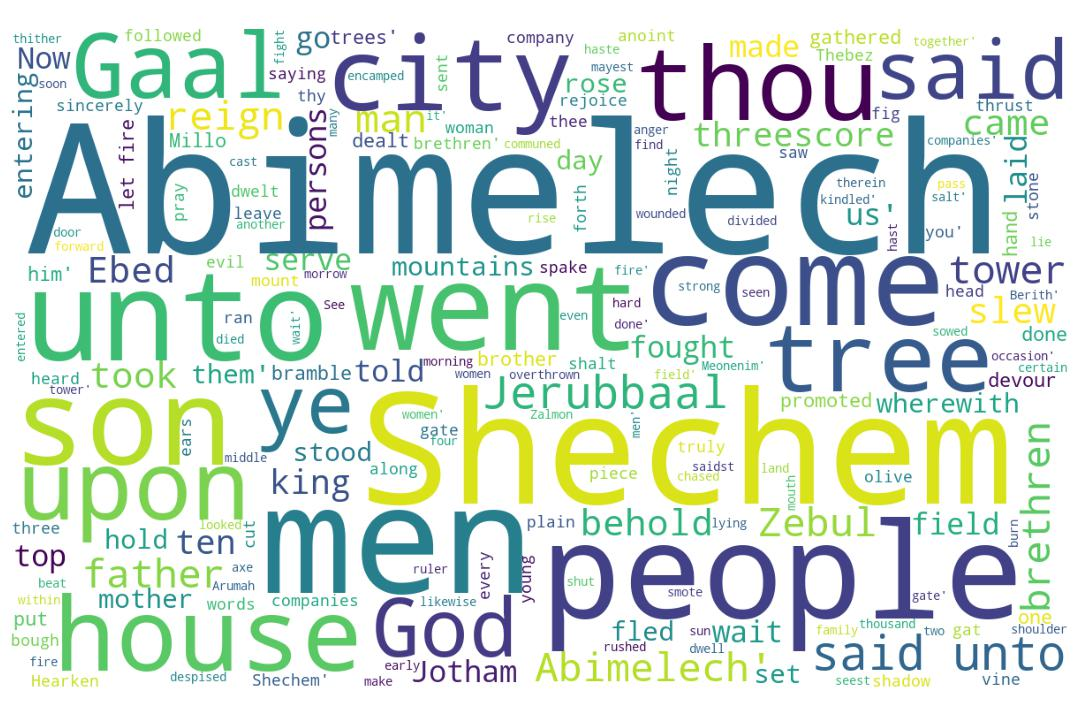
\includegraphics[width=\linewidth]{07OT-Judges/Judges9-WordCloud.jpg}
  \caption{Judges 9 Word Cloud}
  \label{fig:Judges 9 Word Cloud}
\end{figure}

\marginpar{\scriptsize \centering \fcolorbox{bone}{lime}{\textbf{SONS OF GIDEON}}\\ (Judges 9) \begin{compactenum}[I.][8]
    \item  \textbf{Self-Proclaimed} \index[scripture]{Judges!Judges 09:02}(Jdg 9:2)
    \item  \textbf{Seizing Power} \index[scripture]{Judges!Judges 09:02}(Jdg 9:2)
    \item  \textbf{Silver Presented} \index[scripture]{Judges!Judges 09:04}(Jdg 9:4)
    \item  \textbf{Starting the Purge} \index[scripture]{Judges!Judges 09:05}(Jdg 9:5)
    \item  \textbf{Ceremony at the Pillar} \index[scripture]{Judges!Judges 09:06}(Jdg 9:6) -- the place of idolatry
    \item  The \textbf{Story of Punishment} \index[scripture]{Judges!Judges 09:08--21}(Jdg 9:8-21)
    \item  \textbf{Stoned and Put Down} \index[scripture]{Judges!Judges 09:54}(Jdg 9:54)
\end{compactenum}}


\footnote{\textcolor[rgb]{0.00,0.25,0.00}{\hyperlink{JudgesTOC}{Return to end of Table of Contents.}}}\footnote{\href{https://audiobible.com/bible/judges_9.html}{\textcolor[cmyk]{0.99998,1,0,0}{Judges 9 Audio}}}\textcolor[cmyk]{0.99998,1,0,0}{And Abimelech the son of Jerubbaal went to Shechem unto his mother's brethren, and communed with them, and with all the family of the house of his mother's father, saying,}
[2] \textcolor[cmyk]{0.99998,1,0,0}{Speak, I pray you, in the ears of all \fcolorbox{bone}{bone}{the men of Shechem}, Whether \emph{is} better for you, either that all the sons of Jerubbaal, \emph{which} \emph{are} threescore and ten persons, reign over you, or that one reign over you? remember also that I \emph{am} your bone and your flesh.}
[3] \textcolor[cmyk]{0.99998,1,0,0}{And his mother's brethren spake of him in the ears of all \fcolorbox{bone}{bone}{the men of Shechem} all these words: and their hearts inclined to follow Abimelech; for they said, He \emph{is} our brother.}
[4] \textcolor[cmyk]{0.99998,1,0,0}{And they gave him threescore and ten \emph{pieces} of silver out of the house of Baal-berith, wherewith Abimelech hired vain and light persons, which followed him.}
[5] \textcolor[cmyk]{0.99998,1,0,0}{And he went unto his father's house at Ophrah, and slew his brethren the sons of Jerubbaal, \emph{being} threescore and ten persons, upon one stone: notwithstanding yet Jotham the youngest son of Jerubbaal was left; for he hid himself.}
[6] \textcolor[cmyk]{0.99998,1,0,0}{And all \fcolorbox{bone}{bone}{the men of Shechem} gathered together, and all the house of Millo, and went, and made Abimelech king, by the plain of the pillar that \emph{was} in Shechem.}\\
\\
\P \textcolor[cmyk]{0.99998,1,0,0}{And when they told \emph{it} to Jotham, he went and stood in the top of mount Gerizim, and lifted up his voice, and cried, and said unto them, Hearken unto me, ye men of Shechem, that God may hearken unto you.}
[8] \textcolor[cmyk]{0.99998,1,0,0}{The trees went forth \emph{on} \emph{a} \emph{time} to anoint a king over them; and they said unto the olive tree, Reign thou over us.}
[9] \textcolor[cmyk]{0.99998,1,0,0}{But the olive tree said unto them, Should I leave my fatness, wherewith by me they honour God and man, and go to be promoted over the trees?}
[10] \textcolor[cmyk]{0.99998,1,0,0}{And the trees said to the fig tree, Come thou, \emph{and} reign over us.}
[11] \textcolor[cmyk]{0.99998,1,0,0}{But the fig tree said unto them, Should I forsake my sweetness, and my good fruit, and go to be promoted over the trees?}
[12] \textcolor[cmyk]{0.99998,1,0,0}{Then said the trees unto the vine, Come thou, \emph{and} reign over us.}
[13] \textcolor[cmyk]{0.99998,1,0,0}{And the vine said unto them, Should I leave my wine, which cheereth God and man, and go to be promoted over the trees?}
[14] \textcolor[cmyk]{0.99998,1,0,0}{Then said all the trees unto the bramble, Come thou, \emph{and} reign over us.}
[15] \textcolor[cmyk]{0.99998,1,0,0}{And the bramble said unto the trees, If in truth ye anoint me king over you, \emph{then} come \emph{and} put your trust in my shadow: and if not, let fire come out of the bramble, and devour the cedars of Lebanon.}
[16] \textcolor[cmyk]{0.99998,1,0,0}{Now therefore, if ye have done truly and sincerely, in that ye have made Abimelech king, and if ye have dealt well with Jerubbaal and his house, and have done unto him according to the deserving of his hands;}
[17] \textcolor[cmyk]{0.99998,1,0,0}{(For my father fought for you, and adventured his life far, and delivered you out of the hand of Midian:}
[18] \textcolor[cmyk]{0.99998,1,0,0}{And ye are risen up against my father's house this day, and have slain his sons, threescore and ten persons, upon one stone, and have made Abimelech, the son of his maidservant, king over \fcolorbox{bone}{bone}{the men of Shechem}, because he \emph{is} your brother;)}
[19] \textcolor[cmyk]{0.99998,1,0,0}{If ye then have dealt truly and sincerely with Jerubbaal and with his house this day, \emph{then} rejoice ye in Abimelech, and let him also rejoice in you:}
[20] \textcolor[cmyk]{0.99998,1,0,0}{But if not, let fire come out from Abimelech, and devour \fcolorbox{bone}{bone}{the men of Shechem}, and the house of Millo; and let fire come out from \fcolorbox{bone}{bone}{the men of Shechem}, and from the house of Millo, and devour Abimelech.}
[21] \textcolor[cmyk]{0.99998,1,0,0}{And Jotham ran away, and fled, and went to Beer, and dwelt there, for fear of Abimelech his brother.}\\
\\
\P \textcolor[cmyk]{0.99998,1,0,0}{When Abimelech had reigned three years over Israel,}
[23] \textcolor[cmyk]{0.99998,1,0,0}{Then God sent an evil spirit between Abimelech and \fcolorbox{bone}{bone}{the men of Shechem}; and \fcolorbox{bone}{bone}{the men of Shechem} dealt treacherously with Abimelech:}
[24] \textcolor[cmyk]{0.99998,1,0,0}{That the cruelty \emph{done} to the threescore and ten sons of Jerubbaal might come, and their blood be laid upon Abimelech their brother, which slew them; and upon \fcolorbox{bone}{bone}{the men of Shechem}, which aided him in the killing of his brethren.}
[25] \textcolor[cmyk]{0.99998,1,0,0}{And \fcolorbox{bone}{bone}{the men of Shechem} set liers in wait for him in the top of the mountains, and they robbed all that came along that way by them: and it was told Abimelech.}
[26] \textcolor[cmyk]{0.99998,1,0,0}{And Gaal the son of Ebed came with his brethren, and went over to Shechem: and \fcolorbox{bone}{bone}{the men of Shechem} put their confidence in him.}
[27] \textcolor[cmyk]{0.99998,1,0,0}{And they went out into the fields, and gathered their vineyards, and trode \emph{the} \emph{grapes}, and made merry, and went into the house of their god, and did eat and drink, and cursed Abimelech.}
[28] \textcolor[cmyk]{0.99998,1,0,0}{And Gaal the son of Ebed said, Who \emph{is} Abimelech, and who \emph{is} Shechem, that we should serve him? \emph{is} not \emph{he} the son of Jerubbaal? and Zebul his officer? serve the men of Hamor the father of Shechem: for why should we serve him?}
[29] \textcolor[cmyk]{0.99998,1,0,0}{And would to God this people were under my hand! then would I remove Abimelech. And he said to Abimelech, Increase thine army, and come out.}\\
\\
\P \textcolor[cmyk]{0.99998,1,0,0}{And when Zebul the ruler of the city heard the words of Gaal the son of Ebed, his anger was kindled.}
[31] \textcolor[cmyk]{0.99998,1,0,0}{And he sent messengers unto Abimelech privily, saying, Behold, Gaal the son of Ebed and his brethren be come to Shechem; and, behold, they fortify the city against thee.}
[32] \textcolor[cmyk]{0.99998,1,0,0}{Now therefore up by night, thou and \fcolorbox{bone}{bone}{the people} that \emph{is} with thee, and lie in wait in the field:}
[33] \textcolor[cmyk]{0.99998,1,0,0}{And it shall be, \emph{that} in the morning, as soon as the sun is up, thou shalt rise early, and set upon the city: and, behold, \emph{when} he and \fcolorbox{bone}{bone}{the people} that \emph{is} with him come out against thee, then mayest thou do to them as thou shalt find occasion.}\\
\\
\P \textcolor[cmyk]{0.99998,1,0,0}{And Abimelech rose up, and all \fcolorbox{bone}{bone}{the people} that \emph{were} with him, by night, and they laid wait against Shechem in four companies.}
[35] \textcolor[cmyk]{0.99998,1,0,0}{And Gaal the son of Ebed went out, and stood in the entering of the gate of the city: and Abimelech rose up, and \fcolorbox{bone}{bone}{the people} that \emph{were} with him, from lying in wait.}
[36] \textcolor[cmyk]{0.99998,1,0,0}{And when Gaal saw \fcolorbox{bone}{bone}{the people}, he said to Zebul, Behold, there come people down from the top of the mountains. And Zebul said unto him, Thou seest the shadow of the mountains as \emph{if} \emph{they} \emph{were} men.}
[37] \textcolor[cmyk]{0.99998,1,0,0}{And Gaal spake again and said, See there come people down by the middle of the land, and another company come along by the plain of Meonenim.}
[38] \textcolor[cmyk]{0.99998,1,0,0}{Then said Zebul unto him, Where \emph{is} now thy mouth, wherewith thou saidst, Who \emph{is} Abimelech, that we should serve him? \emph{is} not this \fcolorbox{bone}{bone}{the people} that thou hast despised? go out, I pray now, and fight with them.}
[39] \textcolor[cmyk]{0.99998,1,0,0}{And Gaal went out before \fcolorbox{bone}{bone}{the men of Shechem}, and fought with Abimelech.}
[40] \textcolor[cmyk]{0.99998,1,0,0}{And Abimelech chased him, and he fled before him, and many were overthrown \emph{and} wounded, \emph{even} unto the entering of the gate.}
[41] \textcolor[cmyk]{0.99998,1,0,0}{And Abimelech dwelt at Arumah: and Zebul thrust out Gaal and his brethren, that they should not dwell in Shechem.}
[42] \textcolor[cmyk]{0.99998,1,0,0}{And it came to pass on the morrow, that \fcolorbox{bone}{bone}{the people} went out into the field; and they told Abimelech.}
[43] \textcolor[cmyk]{0.99998,1,0,0}{And he took \fcolorbox{bone}{bone}{the people}, and divided them into three companies, and laid wait in the field, and looked, and, behold, \fcolorbox{bone}{bone}{the people} \emph{were} come forth out of the city; and he rose up against them, and smote them.}
[44] \textcolor[cmyk]{0.99998,1,0,0}{And Abimelech, and the company that \emph{was} with him, rushed forward, and stood in the entering of the gate of the city: and the two \emph{other} companies ran upon all \emph{the} \emph{people} that \emph{were} in the fields, and slew them.}
[45] \textcolor[cmyk]{0.99998,1,0,0}{And Abimelech fought against the city all that day; and he took the city, and slew \fcolorbox{bone}{bone}{the people} that \emph{was} therein, and beat down the city, and sowed it with salt.}\\
\\
\P \textcolor[cmyk]{0.99998,1,0,0}{And when all the men of the tower of Shechem heard \emph{that}, they entered into an hold of the house of the god Berith.}
[47] \textcolor[cmyk]{0.99998,1,0,0}{And it was told Abimelech, that all the men of the tower of Shechem were gathered together.}
[48] \textcolor[cmyk]{0.99998,1,0,0}{And Abimelech gat him up to mount Zalmon, he and all \fcolorbox{bone}{bone}{the people} that \emph{were} with him; and Abimelech took an axe in his hand, and cut down a bough from the trees, and took it, and laid \emph{it} on his shoulder, and said unto \fcolorbox{bone}{bone}{the people} that \emph{were} with him, What ye have seen me do, make haste, \emph{and} do as I \emph{have} \emph{done}.}
[49] \textcolor[cmyk]{0.99998,1,0,0}{And all \fcolorbox{bone}{bone}{the people} likewise cut down every man his bough, and followed Abimelech, and put \emph{them} to the hold, and set the hold on fire upon them; so that all the men of the tower of Shechem died also, about a thousand men and women.}\\
\\
\P \textcolor[cmyk]{0.99998,1,0,0}{Then went Abimelech to Thebez, and encamped against Thebez, and took it.}
[51] \textcolor[cmyk]{0.99998,1,0,0}{But there was a strong tower within the city, and thither fled all the men and women, and all they of the city, and shut \emph{it} to them, and gat them up to the top of the tower.}
[52] \textcolor[cmyk]{0.99998,1,0,0}{And Abimelech came unto the tower, and fought against it, and went hard unto the door of the tower to burn it with fire.}
[53] \textcolor[cmyk]{0.99998,1,0,0}{And a certain woman cast a piece of a millstone upon Abimelech's head, and all to brake his skull.}
[54] \textcolor[cmyk]{0.99998,1,0,0}{Then he called hastily unto the young man his armourbearer, and said unto him, Draw thy sword, and slay me, that men say not of me, A woman slew him. And his young man thrust him through, and he died.}
[55] \textcolor[cmyk]{0.99998,1,0,0}{And when the men of Israel saw that Abimelech was dead, they departed every man unto his place.}\\
\\
\P \textcolor[cmyk]{0.99998,1,0,0}{Thus God rendered the wickedness of Abimelech, which he did unto his father, in slaying his seventy brethren:}
[57] \textcolor[cmyk]{0.99998,1,0,0}{And all the evil of \fcolorbox{bone}{bone}{the men of Shechem} did God render upon their heads: and upon them came the curse of Jotham the son of Jerubbaal.}

\chapter{Psalm 75}

\begin{figure}
  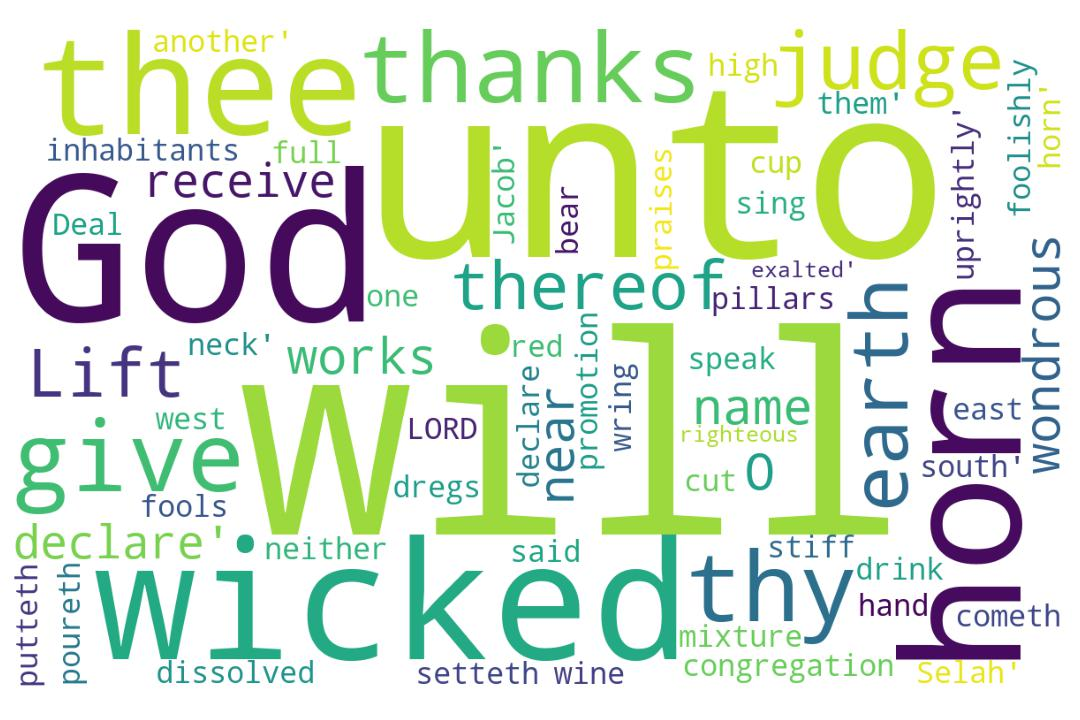
\includegraphics[width=\linewidth]{19OT-Psalms/Psalm75-WordCloud.jpg}
  \caption{Psalm 75 Word Cloud}
  \label{fig:Psalm 75 word Cloud}
\end{figure}

\marginpar{\scriptsize \centering \fcolorbox{bone}{lime}{\textbf{A WORTHY GOD}}\\ (Psalm 75:1-10) \begin{compactenum}[I.][8]
    \item A \textbf{Worthy Declaration} \index[scripture]{Psalms!Psa 075:01}(Psa 75:1)
    \item \textbf{Works on Display} \index[scripture]{Psalms!Psa 075:01}(Psa 75:1)
    \item (Sinful) \textbf{World Dissolved} \index[scripture]{Psalms!Psa 075:03}(Psa 75:3)
    \item \textbf{Weighty Decisions} \index[scripture]{Psalms!Psa 075:07}(Psa 75:7)
     \item A \textbf{Wrathful Drink} (The Cup) \index[scripture]{Psalms!Psa 075:08}(Psa 75:8)
     \item The \textbf{Wringing out of Dregs} \index[scripture]{Psalms!Psa 075:08}(Psa 75:8)
   \item (The) \textbf{Wicked Destroyed} \index[scripture]{Psalms!Psa 075:10}(Psa 75:10)
\end{compactenum}}
    
\marginpar{\scriptsize \centering \fcolorbox{bone}{yellow}{\textbf{THE JUDGMENT}}\\ (Psalm 75:1-10) \begin{compactenum}[I.][8]
    \item The \textbf{Declaration} \index[scripture]{Psalms!Psa 075:01} \index[scripture]{Psalms!Psa 075:09}(Psa 75:1, 9)
    \item \textbf{Dealings} \index[scripture]{Psalms!Psa 075:04} (Psa 75:4)
    \item \textbf{Dissolution} \index[scripture]{Psalms!Psa 075:05} (Psa 75:5)
    \item \textbf{Directions} \index[scripture]{Psalms!Psa 075:06} (Psa 75:6) (Look North!)
    \item \textbf{Dregs} \index[scripture]{Psalms!Psa 075:08} (Psa 75:8) 
    \item The \textbf{Drinking} \index[scripture]{Psalms!Psa 075:08} (Psa 75:8) 
    \item The \textbf{Defeat} \index[scripture]{Psalms!Psa 075:10} (Psa 75:10) 
\end{compactenum}}
    




% \textcolor[cmyk]{0.99998,1,0,0}{
\footnote{\textcolor[rgb]{0.00,0.25,0.00}{\hyperlink{TOC}{Return to end of Table of Contents.}}}\footnote{\href{https://audiobible.com/bible/psalms_75.html}{\textcolor[cmyk]{0.99998,1,0,0}{Psalm 75 Audio}}}\textcolor[cmyk]{0.99998,1,0,0}{To the chief Musician, Al-taschith, A Psalm \emph{or} Song of Asaph.}\\
\\
\textcolor[cmyk]{0.99998,1,0,0}{Unto thee, O God, do we give thanks, \emph{unto} \emph{thee} do we give thanks: for \emph{that} thy name is near thy wondrous \fcolorbox{bone}{lime}{works} declare.}
[2] \textcolor[cmyk]{0.99998,1,0,0}{When I shall receive the congregation I will judge uprightly.}
[3] \textcolor[cmyk]{0.99998,1,0,0}{The earth and all the inhabitants thereof are \fcolorbox{bone}{lime}{dissolved}: I bear up the pillars of it. Selah.}\footnote{\textbf{1 Peter 3:11-12} - Seeing then that all these things shall be dissolved, what manner of persons ought ye to be in all holy conversation and godliness, [12] Looking for and hasting unto the coming of the day of God, wherein the heavens being on fire shall be dissolved, and the elements shall melt with fervent heat?}
[4] \textcolor[cmyk]{0.99998,1,0,0}{I said unto the fools, Deal not foolishly: and to the wicked, Lift not up the horn:}
[5] \textcolor[cmyk]{0.99998,1,0,0}{Lift not up your horn on high: speak \emph{not} \emph{with} a stiff neck.}
[6] \textcolor[cmyk]{0.99998,1,0,0}{For promotion \emph{cometh} neither from the east, nor from the west, nor from the south.}
[7] \textcolor[cmyk]{0.99998,1,0,0}{But God \emph{is} \fcolorbox{bone}{lime}{the judge}: he putteth down one, and setteth up another.}
[8] \textcolor[cmyk]{0.99998,1,0,0}{For in the hand of the LORD \emph{there} \emph{is} a cup, and the wine is red; it is \fcolorbox{bone}{lime}{full of mixture}; and he poureth out of the same: but the dregs thereof, all the wicked of the earth shall \fcolorbox{bone}{lime}{wring} \emph{them} out, \emph{and} drink \emph{them}.}
[9] \textcolor[cmyk]{0.99998,1,0,0}{But I will declare for ever; I will sing praises to the God of Jacob.}
[10] \textcolor[cmyk]{0.99998,1,0,0}{All the horns of the \fcolorbox{bone}{lime}{wicked} also will I cut off; \emph{but} the horns of the righteous shall be exalted.}\footnote{See the horns of \textbf{Revelation 13:1} - And I stood upon the sand of the sea, and saw a beast rise up out of the sea, having seven heads and ten horns, and upon his horns ten crowns, and upon his heads the name of blasphemy. ``Horns'' indicate powers.} 

 \chapter{Proverb 16}
 
\begin{figure}
  \includegraphics[width=\linewidth]{20OT-Proverbs/Proverb16-Wordcloud.jpg}
  \caption{Proverb 16 Word Cloud}
  \label{fig:Proverb 16 word Cloud}
\end{figure}

\marginpar{\scriptsize \centering \fcolorbox{bone}{lime}{\textbf{PRAYERS FOR THE FAITHFUL}}\\ (Proverb 16:1-33) \begin{compactenum}[I.][8]
    \item \textbf{Prepare my Heart}  \index[scripture]{Proverbs!Pro 16:01}(Pro 16:1)
    \item \textbf{Peruse my Ways} \index[scripture]{Proverbs!Pro 16:02}(Pro 16:2)
    \item \textbf{Purify my Thoughts} \index[scripture]{Proverbs!Pro 16:03}(Pro 16:3)
    \item \textbf{Point out the Path} \index[scripture]{Proverbs!Pro 16:09}(Pro 16:9)
    \item \textbf{Passify my Anger} \index[scripture]{Proverbs!Pro 16:14}(Pro 16:14)
    \item \textbf{Preserve my Soul} \index[scripture]{Proverbs!Pro 16:17}(Pro 16:17)
    \item \textbf{Impart Wisdom} \index[scripture]{Proverbs!Pro 16:21}(Pro 16:21)
\end{compactenum}}

\marginpar{\scriptsize \centering \fcolorbox{bone}{yellow}{\textbf{A GODLY MAN}}\\ (Proverb 16:1-33) \begin{compactenum}[I.][8]
    \item Is \textbf{Prepared}  \index[scripture]{Proverbs!Pro 16:01} (Pro 16:1)
    \item Is \textbf{Purposed}  \index[scripture]{Proverbs!Pro 16:03} (Pro 16:3)
    \item Has \textbf{Purged} Iniquity  \index[scripture]{Proverbs!Pro 16:06} (Pro 16:6)
    \item Is \textbf{Peaceable}   \index[scripture]{Proverbs!Pro 16:07} (Pro 16:7)
    \item Is \textbf{Preserved}   \index[scripture]{Proverbs!Pro 16:17} (Pro 16:17)
    \item Is not \textbf{Proud}   \index[scripture]{Proverbs!Pro 16:19} (Pro 16:19)
    \item Is \textbf{Prudent}   \index[scripture]{Proverbs!Pro 16:21} (Pro 16:21)
\end{compactenum}}

\marginpar{\scriptsize \centering \fcolorbox{bone}{black}{\textbf{\textcolor[cmyk]{0,0,0,0}{GOD IN CONTROL}}}\\ (Proverb 16) 
 \begin{compactenum}[I.][8]
	\item \textbf{Determined Spirits} \index[scripture]{Proverbs!Pro 16:09} (Pro 16:9)
	\item \textbf{Directed Steps}  \index[scripture]{Proverbs!Pro 16:09} (Pro 16:9)
	\item A \textbf{Divine Sentence}  \index[scripture]{Proverbs!Pro 16:10}  (Pro 16:10)
	\item \textbf{Destroyed Soul}  \index[scripture]{Proverbs!Pro 16:18}  (Pro 16:18)
	\item A \textbf{Delighted Soul}  \index[scripture]{Proverbs!Pro 16:19}  (Pro 16:19)
	\item \textbf{Dug-up Sorrows}  \index[scripture]{Proverbs!Pro 16:27} (Pro 16:27)
	\item A \textbf{Disciplined Spirit}  \index[scripture]{Proverbs!Pro 16:32} (Pro 16:32)
\end{compactenum}}


\marginpar{\scriptsize \centering \fcolorbox{bone}{blue}{\textbf{\textcolor[cmyk]{0,0,0,0}{DETAILS}}}\\ (Proverb 16) 
 \begin{compactenum}[I.][8]

 	\item The \textbf{Works} \index[scripture]{Proverbs!Pro 16:03}(Pro 16:3)
	\item The \textbf{Wicked} \index[scripture]{Proverbs!Pro 16:04}(Pro 16:4)
	\item The \textbf{Ways} \index[scripture]{Proverbs!Pro 16:07}(Pro 16:7)
	\item The \textbf{Way} \index[scripture]{Proverbs!Pro 16:09}\index[scripture]{Proverbs!Pro 16:17}\index[scripture]{Proverbs!Pro 16:25}\index[scripture]{Proverbs!Pro 16:29}\index[scripture]{Proverbs!Pro 16:31}(Pro 16:9, 17, 25, 29, 31)
	\item The \textbf{Weights} \index[scripture]{Proverbs!Pro 16:11}(Pro 16:11)
	\item The \textbf{Wisdom} \index[scripture]{Proverbs!Pro 16:16}(Pro 16:16)
	\item The \textbf{Wellspring} \index[scripture]{Proverbs!Pro 16:22}(Pro 16:22)
	\item The \textbf{Words} \index[scripture]{Proverbs!Pro 16:24}(Pro 16:24)
	\item The \textbf{Whisperer} \index[scripture]{Proverbs!Pro 16:28}(Pro 16:28)
\end{compactenum}}








\footnote{\textcolor[cmyk]{0.99998,1,0,0}{\hyperlink{TOC}{Return to end of Table of Contents.}}}\footnote{\href{https://audiobible.com/bible/proverbs_16.html}{\textcolor[cmyk]{0.99998,1,0,0}{Proverbs Audio}}}\textcolor[cmyk]{0.99998,1,0,0}{The \fcolorbox{bone}{lime}{preparations of the heart} in man, and the answer of the tongue, \emph{is} from the LORD.}
[2] \textcolor[cmyk]{0.99998,1,0,0}{All the ways of a man \emph{are} clean in his own eyes; but the \fcolorbox{bone}{lime}{LORD} \fcolorbox{bone}{lime}{weigheth} \fcolorbox{bone}{lime}{the} \fcolorbox{bone}{lime}{spirits}.}
[3] \textcolor[cmyk]{0.99998,1,0,0}{Commit thy works unto the LORD, and thy \fcolorbox{bone}{lime}{thoughts shall be} \fcolorbox{bone}{lime}{established}.}
[4] \textcolor[cmyk]{0.99998,1,0,0}{The LORD hath made all \emph{things} for himself: yea, even the wicked for the day of evil.}
[5] \textcolor[cmyk]{0.99998,1,0,0}{Every one \emph{that} \emph{is} proud in heart \emph{is} an abomination to the LORD: \emph{though} hand \emph{join} in hand, he shall not be unpunished.}
[6] \textcolor[cmyk]{0.99998,1,0,0}{By mercy and truth iniquity is purged: and by the fear of the LORD \emph{men} depart from evil.}
[7] \textcolor[cmyk]{0.99998,1,0,0}{When a man's ways please the LORD, he maketh even his enemies to be at peace with him.}
[8] \textcolor[cmyk]{0.99998,1,0,0}{Better \emph{is} a little with \fcolorbox{bone}{MYGOLD}{righteousness} than great revenues without right.}
[9] \textcolor[cmyk]{0.99998,1,0,0}{A man's heart deviseth his way: but the \fcolorbox{bone}{lime}{LORD directeth his steps}.}
[10] \textcolor[cmyk]{0.99998,1,0,0}{A divine sentence \emph{is} in the lips of the king: his mouth \fcolorbox{bone}{MYGOLD}{transgresseth} not in judgment.}
[11] \textcolor[cmyk]{0.99998,1,0,0}{A just weight and balance \emph{are} the LORD'S: all the weights of the bag \emph{are} his work.}
[12] \textcolor[cmyk]{0.99998,1,0,0}{\emph{It} \emph{is} an abomination to kings to commit wickedness: for the throne is established by \fcolorbox{bone}{MYGOLD}{righteousness}.}
[13] \textcolor[cmyk]{0.99998,1,0,0}{Righteous lips \emph{are} the delight of kings; and they love him that speaketh right.}
[14] \textcolor[cmyk]{0.99998,1,0,0}{The wrath of a king \emph{is} \emph{as} messengers of death: but a \fcolorbox{bone}{lime}{wise man will pacify it}.}
[15] \textcolor[cmyk]{0.99998,1,0,0}{In the light of the king's countenance \emph{is} life; and his favour \emph{is} as a cloud of the latter rain.}
[16] \textcolor[cmyk]{0.99998,1,0,0}{How much better \emph{is} \emph{it} to get wisdom than gold! and to get \fcolorbox{bone}{MYGOLD}{understanding} rather to be chosen than silver!}
[17] \textcolor[cmyk]{0.99998,1,0,0}{The highway of the upright \emph{is} to depart from evil: he that keepeth his way \fcolorbox{bone}{lime}{preserveth} his soul.}
[18] \textcolor[cmyk]{0.99998,1,0,0}{Pride \emph{goeth} before destruction, and an haughty spirit before a fall.}
[19] \textcolor[cmyk]{0.99998,1,0,0}{Better \emph{it} \emph{is} \emph{to} \emph{be} of an humble spirit with the lowly, than to divide the spoil with the proud.}
[20] \textcolor[cmyk]{0.99998,1,0,0}{He that handleth a matter wisely shall find good: and whoso trusteth in the LORD, happy \emph{is} he.}
[21] \textcolor[cmyk]{0.99998,1,0,0}{The \fcolorbox{bone}{lime}{wise in heart} shall be called prudent: and the sweetness of the lips increaseth learning.}
[22] \textcolor[cmyk]{0.99998,1,0,0}{\fcolorbox{bone}{MYGOLD}{Understanding} \emph{is} a wellspring of life unto him that hath it: but the instruction of fools \emph{is} folly.}\footnote{\textbf{Proverbs 18:4} - The words of a man’s mouth are as deep waters, and the wellspring of wisdom as a flowing brook.}\marginpar{ \scriptsize  {\textcolor[rgb]{0.00,0.545,0.269}{$\rightarrow$``wellspring'' found ONLY here and in Proverbs 18:4.}}}
[23] \textcolor[cmyk]{0.99998,1,0,0}{The heart of the wise teacheth his mouth, and addeth learning to his lips.}
[24] \textcolor[cmyk]{0.99998,1,0,0}{Pleasant words \emph{are} \emph{as} an honeycomb, sweet to the soul, and health to the bones.}
[25] \textcolor[cmyk]{0.99998,1,0,0}{There is a way that seemeth right unto a man, but the end thereof \emph{are} the ways of death.}
[26] \textcolor[cmyk]{0.99998,1,0,0}{He that laboureth laboureth for himself; for his mouth craveth it of him.}
[27] \textcolor[cmyk]{0.99998,1,0,0}{An ungodly man diggeth up evil: and in his lips \emph{there} \emph{is} as a burning fire.}
[28] \textcolor[cmyk]{0.99998,1,0,0}{A froward man soweth strife: and a whisperer separateth chief friends.}\footnote{\textbf{Proverb 6:14} - Frowardness is in his heart, he deviseth mischief continually; he soweth discord.}\footnote{\textbf{Proverb 6:19} - A false witness that speaketh lies, and he that soweth discord among brethren.}
[29] \textcolor[cmyk]{0.99998,1,0,0}{A violent man enticeth his neighbour, and leadeth him into the way \emph{that} \emph{is} not good.}
[30] \textcolor[cmyk]{0.99998,1,0,0}{He shutteth his eyes to devise froward things: moving his lips he bringeth evil to pass.}
[31] \textcolor[cmyk]{0.99998,1,0,0}{The hoary head \emph{is} a crown of glory, \emph{if} it be found in the way of \fcolorbox{bone}{MYGOLD}{righteousness}.}
[32] \textcolor[cmyk]{0.99998,1,0,0}{\emph{He} \emph{that} \emph{is} slow to anger \emph{is} better than the mighty; and he that ruleth his spirit than he that taketh a city.}
[33] \textcolor[cmyk]{0.99998,1,0,0}{The lot is cast into the lap; but the whole disposing thereof \emph{is} of the LORD.}




\end{document}

